%!TEX TS-program = xelatex
%!TEX encoding = UTF-8 Unicode

\documentclass[12pt]{article} % A4 paper size, default 11pt font size and oneside for equal margins
\usepackage[bottom=2.54cm, left=2.54cm, right=2.54cm, top=2.54cm]{geometry}
\usepackage[english,german]{babel}
\usepackage[toc,numberedsection]{glossaries}
\usepackage[style=alphabetic, citestyle=authoryear,date=iso, urldate=iso]{biblatex}
\usepackage{titlesec}
\usepackage[x11names]{xcolor}
\usepackage{tcolorbox}
\usepackage{scalerel,stackengine,amsmath}
\usepackage{textcomp}
\usepackage[T1]{fontenc}
\usepackage{tikz}
\usepackage{pgfplots}
\usepackage{siunitx}
\usepackage{mathtools}
\usepackage{cancel}
\usepackage{qrcode}
\usepackage{tabularx}
\PassOptionsToPackage{hyphens}{url}
\usepackage{hyperref}
\usepackage{dirtytalk}
\usepackage{float}

\batchmode

\renewcommand*{\nameyeardelim}{\addcomma\space}
\usetikzlibrary{positioning,fit,calc,arrows.meta,arrows}
\usepgfplotslibrary{units}
\newcommand\equalhat{\mathrel{\stackon[1.5pt]{=}{\stretchto{%
    \scalerel*[\widthof{=}]{\wedge}{\rule{1ex}{3ex}}}{0.5ex}}}}

\tikzset{
  labelbox/.style={draw,thick,text width=2.5cm,minimum height=1cm,align=center},
  round/.style={circle,draw,thin, minimum size=5mm},
  emptynode/.style={draw=none},
  arrow_right/.style={-{Latex[length=2mm]}},
  spot/.style={draw,shape=circle,fill=black,inner sep=1.5pt, minimum size = 0.5mm}
}

\pgfplotsset{
  compat=1.16,
  axis_regulator_style/.style={
    width=8.8cm,
    axis x line=center,
    axis y line=left,
    xlabel style={right = 0cm and 0.1cm},
    ylabel style={above left},
    legend cell align={left}
  },
  axis_results_style/.style={
    width=8.8cm,
    axis x line=bottom,
    axis y line=left,
    legend cell align={left}
  },
  line_black/.style={
    color=black!70,
    line width= 1pt
  },
  line_blue/.style={
    color=blue!70,
    line width= 1pt
  },
  line_red/.style={
    color=red!70,
    line width= 1pt
  }
}



\newcommand{\newpara}
{
  \vskip 0.5cm
}
\raggedbottom

\newlength\tindent
\setlength{\tindent}{\parindent}
\setlength{\parindent}{0pt}
\renewcommand{\indent}{\hspace*{\tindent}}

% \usepackage{newtxtext}
% \usepackage{amsmath}
% \usepackage[mathrm=sym]{unicode-math}
% \setmathfont{Fira Math}

%----------------------------------------------------------------------------------------
%	TITLE PAGE
%----------------------------------------------------------------------------------------



\makeglossaries
\loadglsentries{assets/glossar.tex}
\bibliography{literature_and_stuff}

\begin{document} 
\begin{titlepage} % Suppresses headers and footers on the title page

	\centering % Centre everything on the title page
  \vspace*{10mm}
  {\LARGE GEREGELTE} % Title
  \newpara
  {\LARGE WIRBELSTROMBREMSE}
  \vskip 10mm
  


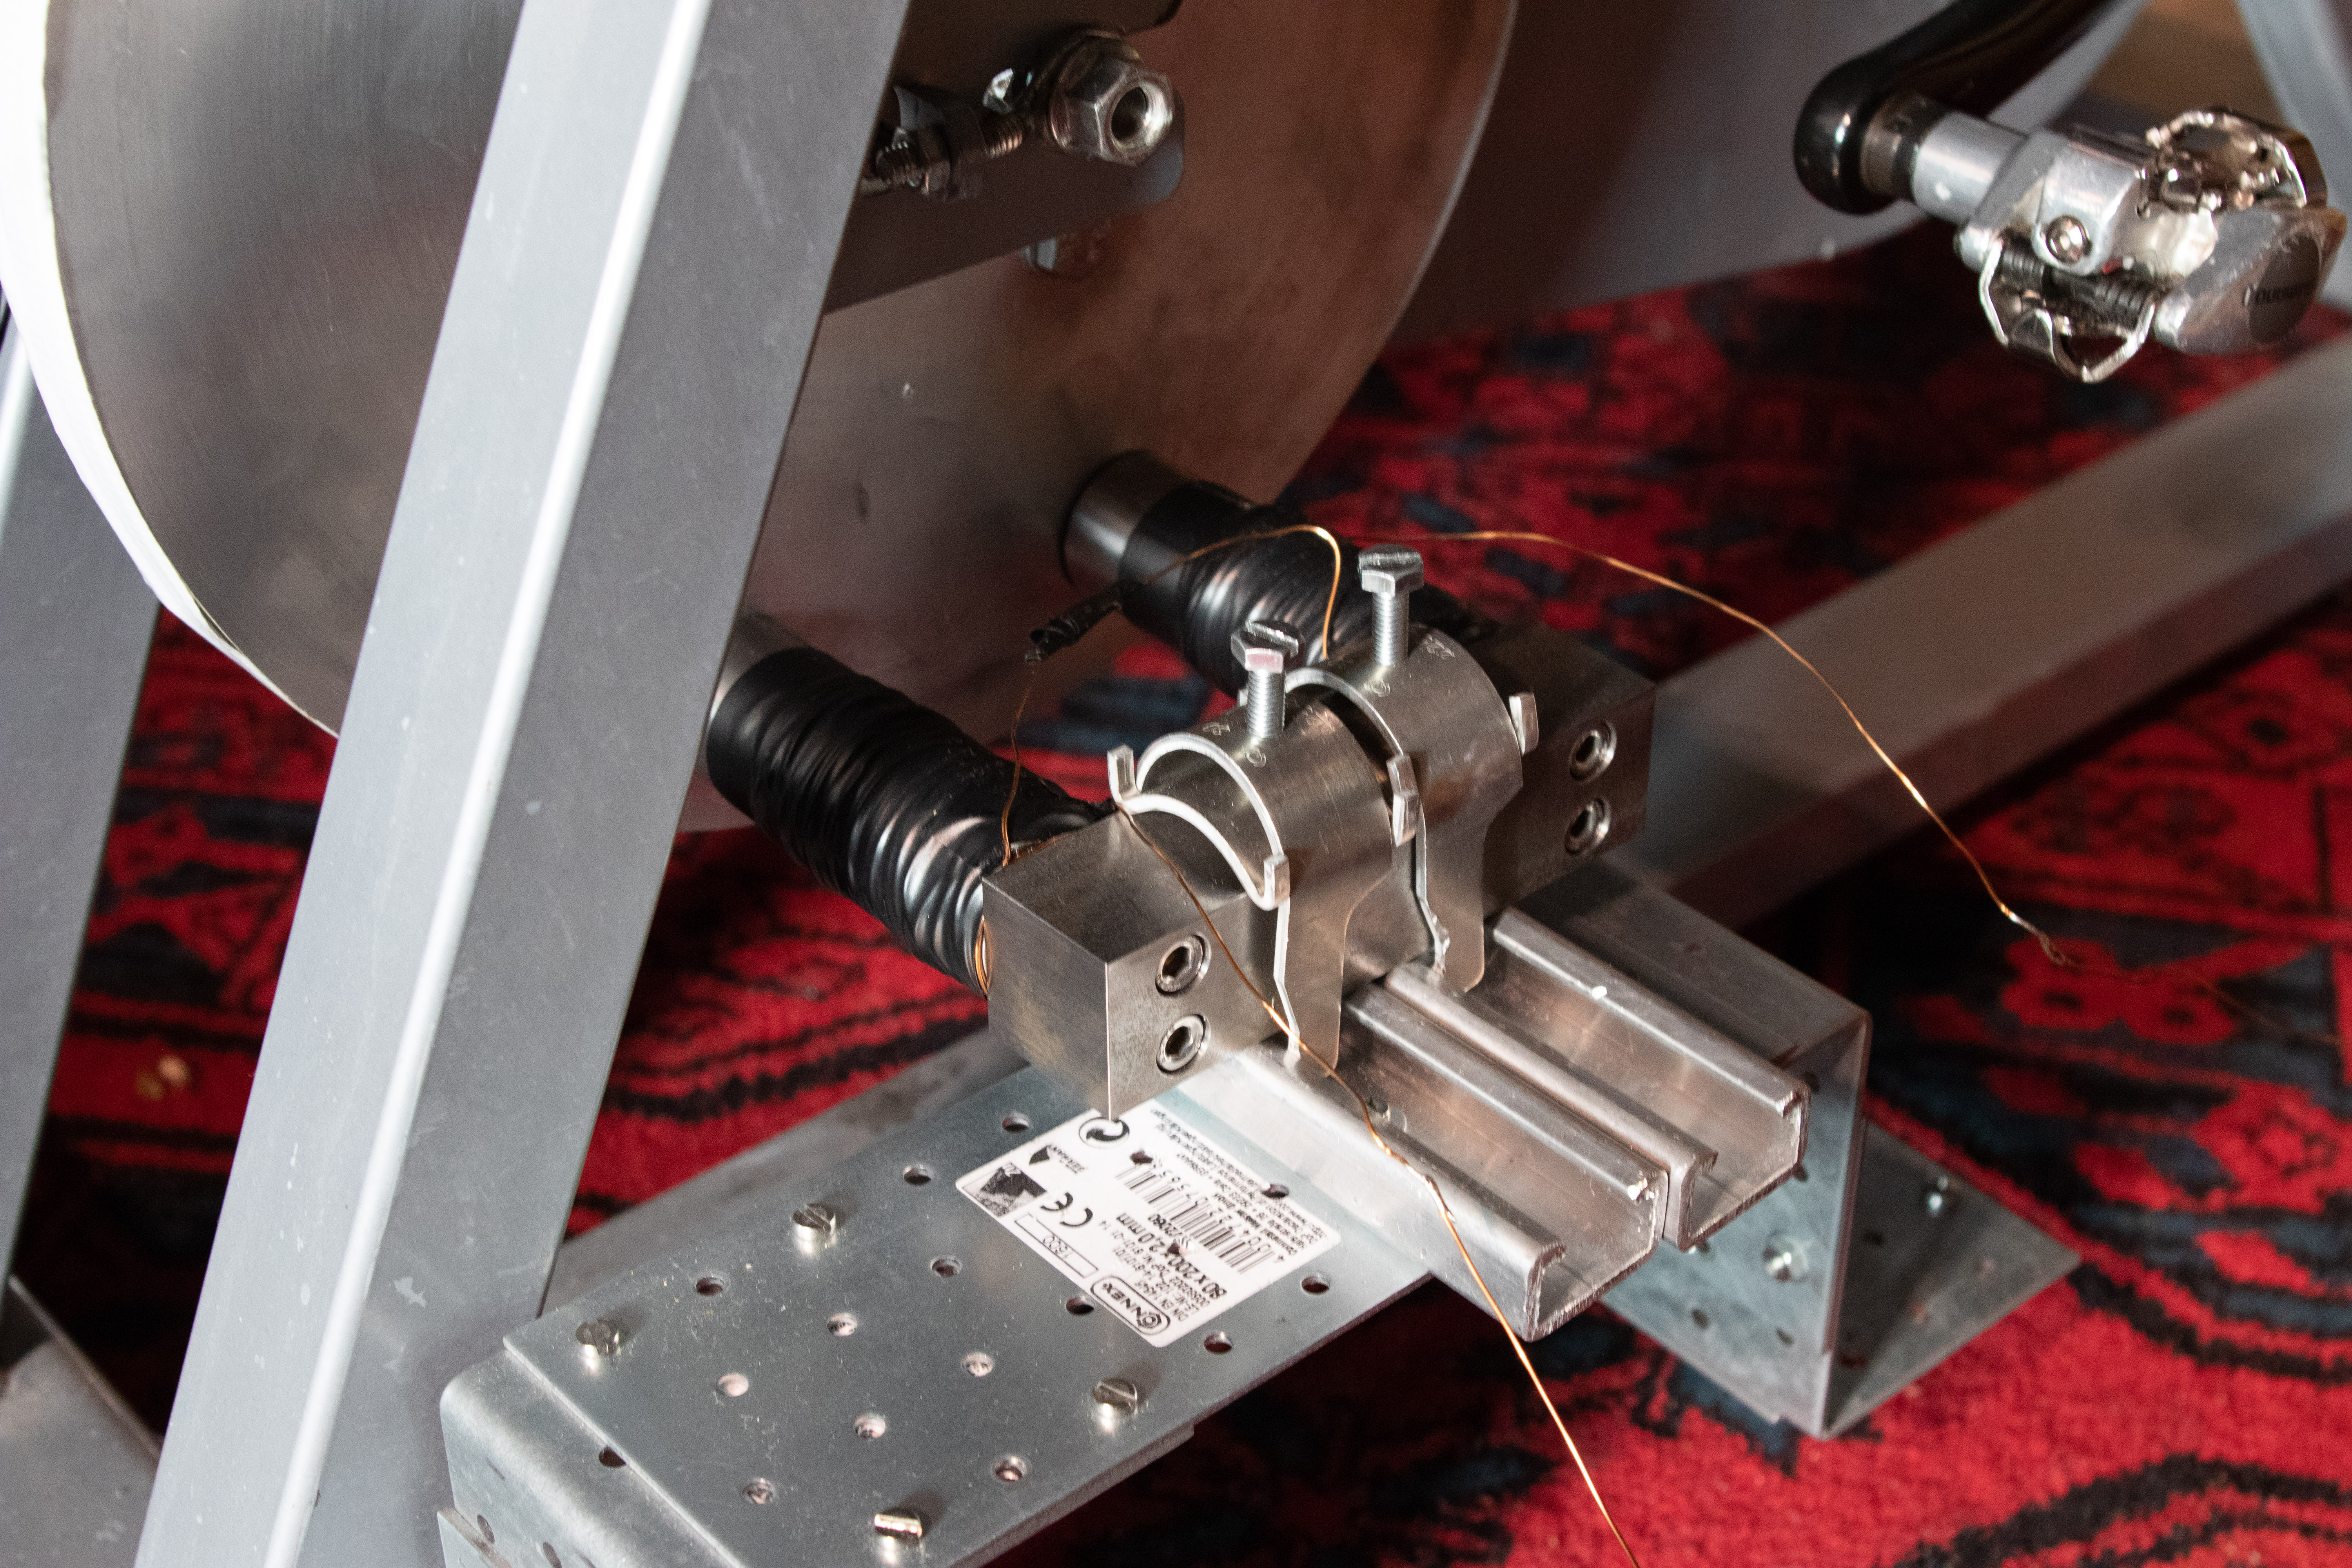
\includegraphics[width=16cm]{assets/images/aufbau}

  {Verfasser}

	{\Large Joel von Rotz \\ Stefan Ruckli \\ \vspace{0.25\baselineskip} Filip Estermann} % Editor list
  \vskip 1cm
    Betreuungslehrperson

    {\large Antonio Russo}
  \vskip 1cm
	\textit{BBZB Luzern} % Editor affiliation
  Februar 2019 % Publication year
	{IDPA-Nr. 1094} % Publisher


\end{titlepage}

%----------------------------------------------------------------------------------------
\author{Joel von Rotz\\Stefan Ruckli\\Filip Estermann}
\date{Februar 2019}
\tableofcontents
\vskip 2cm

\section{Vorwort}
Unsere Projektgruppe bestand aus einem Elektroniker, einem Netzelektriker und einem Elektroinstallateur. Wir haben ein Projekt gewählt, worin jeder seine individuellen beruflichen Fähigkeiten einbringen konnte. Mit der Projekt geregelte Wirbelstrombremse konnte dieses Ansinnen erfüllt werden.
\newpara
Wir bedanken uns bei Antonio Russo, da er sich bereit erklärt hat, uns bei diesem Projekt
zu unterstützen. Bei maxon motor ag, für das zur Verfügungstellen von den Messgeräten und bei
der CKW, für das zur Verfügungstellen von den Bearbeitungsmaschinen und dem Rohmaterial.

\section{Abstract}\label{cap:abstract}
Das Ziel dieses Projektes war, eine Wirbelstrombremse zu bauen, die die Geschwindigkeit eines Rades bis zu fünf Prozent genau regeln kann. Dafür wurde ein Spinning Wheel (ein Fitnesstrainer) umgebaut und mit einem Elektromagneten, als Erzeuger der Bremskraft, erweitert. Dies wurde mit einer elektrisch leitenden Scheibe, die die Bremskraft auf das Rad übertragen soll, und mit einer Messeinrichtung, die die Frequenz, mit der sich das Rad dreht, bestimmt. Ausserdem wurde ein elektronischer Regler, der die Spannungsversorgung des Elektromagneten und dessen Bremskraft regeln soll, erstellt.
\newpara
Nach der Planung und nach den ersten Tests wurde analysiert, wo noch Probleme liegen und was angepasst werden muss: dass das Rad noch zu schwer war und verkleinert werden musste.
\newpara
Nach den entsprechenden Änderungen und Umbauten konnte die Wirbelstrombremse wunschgemäss eingesetzt werden und sie bremste das Rad relativ schnell ab. 
\newpara
Bei der Regelung wurde allerdings festgestellt, dass die Berechnung des Elektromagneten fehlerhaft war. Deshalb konnte die Regelung nicht in Betrieb genommen werden.
\newpara
In den folgenden Seiten erfahren Sie eine Einlesung in die wichtigsten Themen und die Gedanken der Verfasser dieser Arbeit.
\newpage

\section{Einleitung}\label{cap:einleitung}
Eine Wirbelstrombremse nutzt das Magnetfeld des Bremsmagneten aus, um die Bremsscheibe abzubremsen. Da sie nur mit der induktiven (magnetischen) Bremskraft arbeitet, ist sie verschleissfrei, also benötigt keine Bremsklötze.
\newpara
 Die Ziele dieser Arbeit waren, eine gut funktionierende Wirbelstrombremse zu bauen und damit auch die Geschwindigkeit zu regeln. Dazu wurde folgende Hypothese formuliert: Eine Wirbelstrombremse, mit der die Geschwindigkeit auf 5\% Toleranz geregelt wird.
 \newpara
Dafür sollte eine elektrisch leitende Platte am Rad eines Spinning Wheels befestigt werden. Mit möglichst wenig Abstand zur der Platte, damit der magnetische Widerstand so gering wie möglich ist, soll ein Elektromagnet in Hufeisenform befestigt werden. Dieser Elektromagnet soll über einen Spannungsregler mit Spannung versorgt werden. Der Elektromagnet induziert in der elektrisch leitenden Platte eine Spannung, welche die Entstehung von Wirbelströmen und die Verzögerung der Platte zur Folge haben soll. Eine Messeinrichtung, bestehend aus einem Magneten, welcher am Rad befestigt ist, sowie einen Magnetschalter, welcher das vorbeibewegende Magnet erkennt, soll die Umdrehungsfrequenz des Rades bestimmen.
\newpara
Nach der Planung und der Materialbeschaffung wurden die Komponenten wie oben beschrieben zusammengebaut und die ersten Tests wurden vorbereitet. Um sicher zu gehen, dass die gemessenen Ergebnisse stimmen, wurde für die Tests eine zusätzliche Messeinrichtung installiert. Für diese Messeinrichtung wurde ein weisses Band um das Rad geklebt und eine Stelle wurde schwarz markiert. Ein Drehzahlmessgerät soll den Kontrast zwischen der schwarz markierten Stelle und dem weissen Band erkennen. Somit erkennt das Gerät, wann sich das Rad einmal im Kreis gedreht hat. Aus diesen Informationen berechnet es die Frequenz des Rades.
\newpara
Bei den ersten Tests funktionierte die Bremse nicht wunschgemäss. Die Bremsung war nur gering festzustellen. Nach der Fehleranalyse stand fest: Das Rad ist zu schwer und muss verkleinert werden, sodass es an Masse verliert.
\newpara
Nach dieser Anpassung wurde das Spinning Wheel erneut für die Tests aufgebaut. Bei diesen erneuten Tests stellten beide Messeinrichtungen einen deutlichen Unterschied zwischen der Verzögerung des Rades mit aktivierter und deaktivierter Wirbelstrombremse fest.
\newpara
Die Wirbelstrombremse funktionierte jetzt wunschgemäss und der Fokus lag nun auf dem zweiten Ziel, der Regelung. Dafür wurde ein elektronischer Regler erstellt. Dieser Regler vergleicht die am Rad gemessene Frequenz mit einer am Regler einstellbaren Frequenz. Anhand von diesen beiden Werten ermittelt der Regler, ob und wie stark das Rad abgebremst werden muss. Der Regler soll dann die Spannungsversorgung des Elektromagneten bestimmen: Muss das Rad stärker abgebremst werden, wird eine höhere Spannung an den Magneten angelegt. Durch die höhere Spannung soll der Elektromagnet eine höhere Bremskraft auf das Rad haben.
\newpara
Der Regler wurde in der Messeinrichtung und in der Spannungsversorgung eingebaut und das Spinning Wheel wurde erneut für die Tests aufgebaut. Die Tests ergaben, dass die Regelung nicht wunschgemäss funktionierte. Der Fehler lag bei der Dimensionierung des Elektromagneten. Dieser lieferte auf die von Konstantstromquelle gespiesene Spannung keine zufriedenstellenden Resultate.
\newpage
\section{Einlesung}\label{cap:einlesung}
\subsection{Magnetismus}\label{cap:einlesung_magnetismus}
Magnetische Felder ist für das menschliche Auge nicht sichtbar und trotzdem finden sie ein weites Spektrum an Anwendungsmöglichkeiten in unserer heutigen Gesellschaft. Magnetische Felder dienen zum Beispiel für den Kompass, da die Felder die Nadel immer nach Norden zeigen lässt, oder für Lautsprecher, damit anhand Schwingungen, welche das Magnetische Feld erzeugt, elektrische Signale zu akustischen Signalen umgewandelt werden können.
\newpara
In den folgenden Unterkapiteln wird die Beeinflussung des Magnetfeldes von verschiedenen Metallen und die Erzeugung eines Magnetfeldes durch den elektrischen Strom erklärt.
\subsubsection{Metalle und deren Magnetfeld}
Eisen gilt als ein Metall, welches ein eigenes Magnetfeld erzeugen kann, indem es in Kontakt mit einem Magnet kommt. Ein Metall, welches ein starkes Magnetfeld erhalten kann, wird als magnetisierbar oder in der Physik als ferromagnetisch bezeichnet.
\newpara
Wird ein Eisen-Stück magnetisiert, entstehen zwei Magnetpole: Norden und Süden. Diese Magnetpole dienen nicht zum Herausfinden des Nord- und Südpols, sondern dienen zum Bestimmen der magnetischen Feldlinien (Siehe Abbildung \ref{fig:magnetismus_polarisation_feldlinien}).
\begin{figure}[ht]
  \begin{center}
    \includegraphics[width=9cm]{assets/images/magnetismus/magnet}
  \end{center}
  \vspace{-3ex}
  \caption{Pole \& Feldlinien eines Magnets}
  \label{fig:magnetismus_polarisation_feldlinien}
\end{figure}

Diese Feldlinien machen wichtige Informationen sichtbar, zum Beispiel wie das Magnetfeld orientiert ist, wie das Magnetfeld von anderen Magnetfeldern beeinflusst wird oder wie stark das Magnetfeld ist (Siehe Abbildung \ref{fig:magnetismus_feldlinien}). Die Stärke wird dabei anhand der Ausbreitung der Feldlinien dargestellt.

\begin{figure}[ht]
    \begin{center}
      \includegraphics[width=10cm]{assets/images/magnetismus/beeinflussungen_magnet}
    \end{center}
    \vspace{-3ex}
    \caption{Darstellung von Feldlinien}
\label{fig:magnetismus_feldlinien}
\end{figure}

Wie vorher erwähnt, geben Feldlinien an, wie stark ein Magnetfeld sein kann, aber wie kann ein starkes Magnetfeld aufgebaut werden? Das Magnetfeld wird durch die Permeabilität beeinflusst, welche je nach Metall verschieden ist. 
\newpara
Die Permeabilitätszahl kann angeben, ob das Metall magnetisch oder nichtmagnetisch ist. Ein Magnet, welches aus Eisen besteht (Permeabilitätszahl = $300…10’000$) wird nicht dasselbe Magnetfeld eines Aluminium-Magneten (Permeabilitätszahl = $1 + 2.2 \cdot 10^{-5}$) sein, da die Permeabilitätszahl sich untereinander stark unterscheiden. Es kann daher bereits durch Betrachtung der Permeabilität der Metalle herausgefunden werden, ob das Metall magnetisch oder nichtmagnetisch ist. Ein typischer Bereich der Permeabilitätszahl von ferromagnetischen Metallen beträgt $300…10’000$. 
\newpage

\subsubsection{Wirbelstrom}

Der Effekt von Wirbelstrom ist bereits in heutigen grossen Transportmitteln weit verbreitet. Heutige Züge sind, neben normalen Bremsen, mit Wirbelstrombremsen ausgestattet (Siehe Abbildung). Dies ermöglicht den Zügen steile Gefälle befahren zu können, ohne die normalen Bremsen verwenden zu müssen. Lastwagen verwenden ebenfalls Wirbelstrombremsen um bei Gefällen nicht ausser Kontrolle zu geraten (\cite{lokifahrer}).
\begin{figure}[ht]
    \begin{center}
      \includegraphics[width=10cm]{assets/images/magnetismus/zug_wirbelstrombremse}
    \end{center}
    \vspace{-3ex}
    \caption{Wirbelstrombremse eines Zuges. Heruntergeladen von \url{http://www.lokifahrer.ch/Lukmanier/Rollmaterial/Bremse/Verschleisslos.htm}}
    \label{fig:zug_wirbelstrombremse}
\end{figure}

Der Wirbelstrom zeigt seinen Effekt nur wenn ein Magnet über eine Platte oder eine drehende Scheibe gezogen wird. Damit nicht zu physikalisch gesprochen wird, wird der Wirbelstrom anhand einem Schlittenbeispiel erklärt. Im folgenden Beispiel wird der Wirbelstrom als die Füsse, welche zum Bremsen verwendet werden, repräsentiert und die Strecke als Elektronenfluss.
\newpara
Man sitzt auf einem Schlitten und fährt eine Strecke herunter. Die Geschwindigkeit des Schlittens erhöht sich konstant, bis es zu schnell wird. Nun drückt man mit den Füssen in den Schnee, um die Geschwindigkeit zu verringern. Man drückt mit der Kraft, welche von den Füssen eingewirkt wird, in den Schnee, was zu einer Reibung und zur Bremsung führt.
\newpara
Wirbelstrom ist also eine Art Energie, welche beim Eindrücken eines Magnetfeldes in eine elektronisch leitfähige Platte erzeugt wird. Der Bremseffekt wird durch \textit{Hineingreifen} des Elektronenflusses erzeugt, was zur Reibung und Bremsung führt (\cite{schulmaterial_magnetismus}). 
\newpage
\subsubsection{Elektromagnetismus}
\say{Elektromagnetismus ist ein Teilgebiet der Physik, das als Elektrodynamik bezeichnet wird.}(\cite{ChemgarooMagnetfelder})
\newpara
Ein Hauptteil der Elektrodynamik beschreibt, dass ein Magnetfeld aufgebaut werden kann, indem elektrischer Strom durch einen Leiter fliesst. Abbildung \ref{fig:rechte_hand_regel} zeigt die Ausrichtung des Magnetfelds bei einem stromdurchflossenem Leiter und eine Darstellung mit der \textit{Rechte-Hand} Regel. Der Daumen zeigt in die Richtung des Stromflusses und die restlichen Finger greifen um den Leiter, was als Magnetfeld bezeichnet wird (\cite{schulmaterial_magnetismus}).

\begin{figure}[ht]
    \begin{center}
      \includegraphics[width=10cm]{assets/images/magnetismus/magnetfeld-leiter-rechte-hand-regel}
    \end{center}
    \vspace{-3ex}
    \caption{Rechte-Hand Regel. Heruntergeladen von \url{https://www.grund-wissen.de/physik/elektrizitaet-und-magnetismus/magnetismus.html}}
    \label{fig:rechte_hand_regel}
\end{figure}

\newpara
Wird ein Kupferkabel, welches um ein Eisenstück gewickelt wurde, mit Strom versorgt, entsteht einen grossen magnetischen Fluss, welcher durch das Eisenstück fliesst (Siehe Abbildung \ref{fig:kupferspule} folgende Seite). Dabei ist zu bemerken, dass sich der Fluss (Abbildung \ref{fig:kupferspule} folgende Seite rechts) jeder Windung zusammensummiert, da alle in die gleiche Richtung fliessen.
\begin{figure}[ht]
    \begin{center}
      \includegraphics[width=8cm]{assets/images/magnetismus/flussrichtung}
    \end{center}
    \vspace{-3ex}
    \caption{Magnetfluss bei einer Kupferspule}
    \label{fig:kupferspule}
\end{figure}
\newpara
Die Stärke ist bei einem elektrischen Magnet von der Stromstärke und der Anzahl Windungen abhängig (Formel \ref{equ:magnetische_durchflutung_einlesung}). Die Stromstärke dient zur Berechnung der magnetischen Kräfte der einzelnen Windungen. Die Windungszahl wird als Faktor für die magnetischen Kräfte verwendet.
\newpage
\begin{equation}
\label{equ:magnetische_durchflutung_einlesung}
\Theta = N\cdot I
\end{equation}
\begin{gather}
\shortintertext{\textbf{Begriffe:}}
\begin{tabularx}{0.9\textwidth}{ll}
$N$	 &  Anzahl Windungen der Wicklung\\
$I$	 &  elektrische Stromstärke
\end{tabularx}\nonumber
\end{gather}
(\cite[S.452]{kuchling2014taschenbuch})
\begin{comment}
Das magnetische Feld ist die Schlüssel-Komponente der Wirbelstrombremse. Fliesst durch eine, sich drehende Scheibe, ein Magnetfeld, so bewirkt diese eine Elektronenbewegung innerhalb der Scheibe aus. Diese Elektronenbewegung lässt die, in unserem Fall nicht ferromagnetische Scheibe, magnetisch werden. Dies bedeutet, dass sich in der Scheibe nun um das Magnetfeld ein, sich kräftemässig entgegengesetztes Magnetfeld entsteht. Diese Eigenschaft kommt der Wirbelstrombremse zugunsten, welche die Scheibe somit kontinuierlich abbremsen lässt.
\newpara


\begin{figure}[ht]
    \begin{center}
      \includegraphics[width=12cm]{assets/images/Eddy_currents_de}
    \end{center}
    \vspace{-3ex}
    \caption[Wirbelstrombremse auf einer Metallplatte]{\centering{Wirbelstrombremse auf einer Metallplatte. Heruntergeladen von \texttt{https://de.wikipedia.org/wiki/Wirbelstrombremse}}}
    \label{fig:eddy_current}
  \end{figure}
\vskip 1cm
Der Wirbelstrom, der sich von der Bewegungsrichtung aus hinter dem Magnet befindet, dreht sich gegen den Uhrzeigersinn. So entsteht ein Magnetfeld in der, sich bewegenden Scheibe, welches mit dem Südpol zum Nordpol schaut. Diese Anziehungskraft wirkt gegen die Bewegung der Scheibe. Der andere Elektronenbewegung, die sich im selben Moment vor dem Magnet befindet, dreht sich allerdings mit dem Uhrzeigersinn. Hier entsteht Ein Magnetfeld, welcher Nordpol sich zum Nordpol des Magneten richtet. Diese Abstossung erzielt ebenso eine Kraft, welche eine Verzögerung auf der Scheibe als Folge hat.
\newpara
Die Scheibe weist eine umso besseren Bremseigenschaft auf, je höher das verwendete Material der Scheibe, den elektrischen Strom leitet. Dies kann damit erklärt werden, da ein Metall, welches einen geringen Widerstand besitzt, viele freie Elektronen mit sich bringt. Somit können auch dementsprechend höhere Wirbelströme entstehen, welche die Scheibe wiederrum bremsen. Die Bremsen erhalten anderseits auch durch Erhöhung des magnetischen Flusses an stärkeren Bremseigenschaften. Durch eine Verringerung des Abstandes, der zwischen Magnet und Scheibe herrscht, kann ebenfalls eine höhere Verzögerung erzielt werden. Die Bremsung erfolgt nicht optimal, wenn der Magnet sich am äussersten Punkt verläuft. Bessere Ergebnisse werden erzielt, wenn sich der Magnet ein wenig tiefer, im Radius befindet. Dies ist indem zu erklären, dass sich andernfalls kein vollständiger Wirbelstrom entstehen kann, welches auch eine schwächere Bremsung als Folge trägt.
\newpara
Prinzipiell ist eine Wirbelstrombremse nicht in der Lage, ein Rad zum Stillstand zu bringen. Um eine Brems-Wirkung zu erzielen, muss bei dieser Wirbelstrombremse eine Elektronenbewegung vorhanden sein, welche kurz vor dem Stillstand noch kaum vorhanden ist. Deshalb bremst dieser, die Scheibe in diesem Punkt so gut wie nicht mehr.
\end{comment}
\subsection{Physik}\label{cap:einlesung_physik}
\subsubsection{Drehmoment}
Bei einer Bremsung wird kinetische Energie in eine andere Energieform, meistens Wärmeenergie, umgewandelt. Durch diese Energieumwandlung sinkt die Geschwindigkeit des zu bremsenden Objektes (\cite{drehmoment}).
\newpara
Eine Geschwindigkeitsänderung im Verhältnis zu der dafür benötigten Zeit wird als Beschleunigung bezeichnet. 
\newpara
Eine Kraft setzt sich aus der Beschleunigung multipliziert mit der beschleunigten Masse zusammen. Daraus folgt: Je grösser die eingesetzte Kraft ist, desto grösser ist die Beschleunigung.
Da diese Kraft auf einen drehbaren, starren Körper ausgeübt wird, wird ein Drehmoment erzeugt. Ein Drehmoment ist das Produkt einer Kraft und dem senkrechten Abstand zum Drehpunkt. Die Wirkung eines Drehmoments entspricht der eines Kräftepaars. Das heisst, je grösser das Drehmoment ist, desto grösser ist seine Kraftwirkung.
\newpara
Aus diesen Erkenntnissen ergibt sich, dass die Position und die Kraft der Bremse eine wichtige Rolle spielen. Um aufgrund des Drehmoments eine optimale negative Beschleunigung zu erzeugen, sollte die Bremse deshalb möglichst weit von der Drehachse entfernt sein und die Kraft, welche im Falle der Wirbelstrombremse von Magneten erzeugt wird, sollte möglichst gross sein. Es spielen aber auch noch andere Faktoren wie die Induktion eine Rolle, wo die Bremse optimalerweise positioniert wird. Deshalb darf sie nicht ganz am Rand der zu bremsenden Scheibe sein (\cite{kuchling2014taschenbuch}).
\subsection{Regler} \label{cap:einlesung_regler}
Regeln ist ein Vorgang, bei dem die Ausgangsgrösse, eine physikalische Grösse wie zum Beispiel die Drehzahl eines Rades, konstant überwacht und bei Abweichungen von einem Sollwert durch die Stellgrösse korrigiert wird (\cite{regelungstechnik}). Die Regelungstechnik ist sehr nützlich für Funktionen, welche einen Zustand konstant behalten müssen, wie zum Beispiel eine Heizung, die 25°C konstant heizen muss. Verändert sich die Temperatur zu 23°C, muss die Heizung das Heizelement erhitzen, um wieder auf 25°C zu kommen. Ist die Temperatur 27°C, muss die Heizung das Heizelement abkühlen lassen.

\begin{figure}[ht]
  \begin{center}
    \begin{tikzpicture}
      \node[labelbox]     (mess)                                          {Messen};
      \node[labelbox]     (verg)  [below right= 3cm and 0.5cm of mess]    {Vergleichen};
      \node[labelbox]     (stel)  [below left = 3cm and 0.5cm of mess]    {Stellen};

      \node[emptynode]    (nod0)  [below right= 0.2cm and 0.2cm of mess]  {};
      \node[emptynode]    (nod1)  [above      = 0.2cm of verg]            {};
      \node[emptynode]    (nod2)  [      left = 0.2cm of verg]            {};
      \node[emptynode]    (nod3)  [      right= 0.2cm of stel]            {};
      \node[emptynode]    (nod4)  [above      = 0.2cm of stel]            {};
      \node[emptynode]    (nod5)  [below left = 0.2cm and 0.2cm of mess]  {};

      \draw [arrow_right] (nod0) -- (nod1);
      \draw [arrow_right] (nod2) -- (nod3);
      \draw [arrow_right] (nod4) -- (nod5);

    \end{tikzpicture}
  \end{center}
  \vspace{-3ex}
  \caption{Regler Blockdiagramm}
  \label{fig:regulator_circulation}
\end{figure}

Die Funktion des Reglers kann in drei Funktionsblöcke eingeteilt werden, welche miteinander interagieren: \textbf{Messen}, \textbf{Vergleichen} und \textbf{Stellen} (Siehe Abbildung \ref{fig:regulator_circulation}). Im Funktionsblock  \textit{Messen} übersetzt ein Sensor die physikalische Grösse in ein Format, welches die Elektronik verstehen kann. Unter \textit{Verstehen} gilt das Umwandeln und Bereitstellen brauchbarer Informationen, wie zum Beispiel die Umwandlung einer Umdrehung eines Rades zu der Zeit, welche dafür benötigt wurde. Im Block \textit{Vergleichen} wird der gemessene Wert mit dem Sollwert verglichen (Siehe Formel \ref{equ:regulator_error}). Die Differenz wird die Regeldifferenz oder auch Regelabweichung, welche im Regler verarbeitet wird. Daraus entsteht die Regelausgangsgrösse, welche in den Aktor geführt wird. Schlussendlich wird im Block \textit{Stellen} aus der Ausgangsgrösse die Stellgrösse mit dem Aktor bestimmt, was zur Veränderung der physikalischen Grösse führt. Durch die Veränderung wird wieder ein neuer Wert gemessen und der gesamte Prozess beginnt von vorne (Siehe Abbildung \ref{fig:regulator_block})(\cite{regelungstechnik}).
\newpage
\begin{equation}
  \label{equ:regulator_error}
  e = w-r
\end{equation}
\begin{gather}
  \shortintertext{\textbf{Begriffe:}}
  \begin{tabularx}{0.9\textwidth}{ll}
    $w$ & Sollwert\\
    $r$ & Istwert\\
    $e$ & Regelabweichung, Regeldifferenz
  \end{tabularx}\nonumber
\end{gather}

\begin{figure}[ht]
  \begin{center}
    \begin{tikzpicture}
      \node[emptynode]    (soll)                                {};
      \node[round]        (diff)        [right=1cm of soll]     {};
      \node[labelbox]     (regl)        [right=1cm of diff]     {Regler};
      \node[labelbox]     (akto)        [right=1cm of regl]     {Aktor};
      \node[labelbox]     (sens)        [below=1cm of akto]     {Sensor};
      \node[labelbox]     (stre)        [right=1cm of akto]     {Regelstrecke};
      \node[emptynode]    (gone)        [right=2cm of stre]     {};
      \node[emptynode]    (erro)        [above=1cm of stre]     {z};
      \node[emptynode]    (minus_diff)  [below right = -1mm and -1mm of diff] {$-$};
      %\node[emptynode]    (plus_diff)   [above left  = -1mm and -1mm of diff] {$+$};
      \node[spot]         (midl)        [right=1cm of stre]     {};


      \draw [arrow_right] (soll)      -- node[above left = 0cm and 1mm]   {$w$} (diff);
      \draw [arrow_right] (diff)      -- node[above left = 0cm and -1mm]  {$e$} (regl);
      \draw [arrow_right] (regl)      -- node[above]                      {$m$} (akto);
      \draw [arrow_right] (akto)      -- node[above]                      {$y$} (stre);
      \draw [-]           (stre)      -- node[above left]                 {$x$} (gone);
      \draw [arrow_right] (midl.center) |-                                      (sens.east);
      \draw [arrow_right] (sens.west) -| node[above left  = 1cm and 0cm]  {$r$} (diff.south);
      \draw [arrow_right] (erro)      --                                            (stre);
    \end{tikzpicture}
  \end{center}
  \vspace{-3ex}
  \caption{Regler Blockdiagramm}
  \label{fig:regulator_block}
\end{figure}
\begin{gather}
  \shortintertext{\textbf{Begriffe:}}
  \begin{tabularx}{.9\textwidth}{cl}
      $w$ & Sollwert\\
      $r$ & Istwert\\
      $e$ & Regelabweichung, Regeldifferenz\\
      $m$ & Regelausgangsgrösse (Befehl von Regler)\\
      $y$ & Stellgrösse (bewirkt eine Änderung der Regelgrösse)\\
      $x$ & Regelgrösse (physikalische Grösse \textrightarrow km/h, rpm, °C, etc.)\\
      $z$ & Störgrösse (beeinflusst die Regelgrösse \textrightarrow °C, von aussen wirkende Kraft)
  \end{tabularx}\nonumber
\end{gather}

\subsubsection{PID-Regler} \label{cap:information_pid_regulator}
In der Wirbelstrombremse war ein PID-Regler geplant, welcher anhand von Geschwindigkeitsmessungen die Stärke des Magneten ansteuert. PID-Regler steht für \textbf{P}roportional-\textbf{I}ntegral-\textbf{D}ifferenzial-Regler und basiert auf mathematische Funktionen (\cite{schulmaterial_regler}).  
\newpara
Was genau diese Funktionen für einen Nutzen haben, wird in den folgenden vier Kapiteln erklärt.
\newpage

\subsubsection{Proportionalität}
Der P-Anteil (Proportionalität) gilt als Hauptregler der drei Funktionen und berücksichtigt die Abweichung zwischen Istwert und Sollwert, in dieser Arbeit ist es die Differenz zwischen der gewünschten Maximalgeschwindigkeit und der aktuellen Geschwindigkeit. Diese Abweichung wird mit dem Faktor $K_P$ multipliziert (Siehe Formel \ref{equ:p_regulator_out}) (\cite{schulmaterial_regler}).

\begin{equation}
  \label{equ:p_regulator_out}
  P_{OUT}=e\cdot K_P
\end{equation}
Der Faktor $K_P$ gibt an, wie stark der Regler bei Abweichungen reagieren soll. Je grösser der Faktor, desto stärker reagiert der Regler (\cite{schulmaterial_regler}). Dieser Faktor lässt dem System zu, das Rad bei Überschreitung der Maximalgeschwindigkeit abzubremsen. Der Nachteil daran ist, dass durch die Verkleinerung der Abweichung auch der P-Anteil kleiner wird, was heisst, dass das Rad nie genau auf die Maximalgeschwindigkeit gebremst werden kann. 
\newpara
Folgende Abbildung (Abbildung \ref{fig:plot_p_regulator_no_feedback}) stellt die Proportionalität bei einer konstanten Abweichung grob dar.

\begin{figure}[h]
  \begin{center}
    \begin{tikzpicture}
      \begin{axis}[
        axis_regulator_style,
               %title         = P-Regler mit konstanter Abweichung,
               ylabel         = {},
        ylabel near ticks, 
        yticklabel pos        = left,
        minor      grid style = {dashed,gray},
                   ymax       = 2,
                   ymin       = -0.5,
                   xmax       = 110,
                   xticklabels    = {,,},
                   xlabel     = {t},
        legend     style      = {draw=none}
      ]
      
        \addplot[line_red] table[x= time,y= e,col sep=comma,mark=none]{assets/diagramm/p_regler_nf.csv}; 
        \addlegendentry{Abweichung}
      
        \addplot[line_blue] table[x= time,y= p,col sep=comma,mark=none]{assets/diagramm/p_regler_nf.csv}; 
        \addlegendentry{Proportionalität}
      \end{axis}
    \end{tikzpicture}
  \end{center}
  \vspace{-3ex}
  
  \caption{P-Regler mit konstanter Abweichung}
  \label{fig:plot_p_regulator_no_feedback}
\end{figure}

Abbildung \ref{fig:plot_p_regulator_controlled} stellt nun die Proportionalität mit einer sich anpassenden Abweichung dar. In dieser Art würde man es in realen Experimenten sehen. Es kann nun der Nachteil der Proportionalität erkannt werden. In diesem Fall ist der $K_P$ Faktor = 0.5, also 50\% der Abweichung, was dazu führt, dass die Abweichung nie den Wert 0 erreichen wird, sondern sehr nahe an 0 kommen wird.

\begin{figure}[h]
  \begin{center}
    \begin{tikzpicture}
      \begin{axis}[
        axis_regulator_style,
               %title      = P-Regler mit konstanter Abweichung,
               ylabel     = {},
        ylabel near ticks, 
        yticklabel pos        = left,
        minor      grid style = {dashed,gray},
                   ymax       = 2,
                   ymin       = -0.5,
                   xmax       = 110,
                   xticklabels    = {,,},
                   xlabel     = {t},
        legend     style      = {draw=none}
      ]
      
        \addplot[line_red] table[x=time,y=e,col sep=comma,mark=none]{assets/diagramm/p_regler_gesteuert.csv};      
        \addlegendentry{Abweichung}
        
        \addplot[line_blue] table[x=time,y=p,col sep=comma,mark=none]{assets/diagramm/p_regler_gesteuert.csv}; 
        \addlegendentry{Proportionalität}
      \end{axis}
    \end{tikzpicture}
  \end{center}
  \vspace{-3ex}
  
  \caption{P-Regler mit Rückkopplung}
  \label{fig:plot_p_regulator_controlled}
\end{figure}
\newpara
\begin{tcolorbox}
  \textbf{\textit{Hinweis:}} Die Grösse der Proportionalität kann verschiedene Formate annehmen. In diesem Fall besitzt die Proportionalität kein Format sondern wird nur als eine simple Zahl dargestellt. Die Proportionalität wird im Nachhinein auf den Aktor angepasst. Dasselbe gilt für die Diagrammen des Integrals und des Differenzials.
\end{tcolorbox}
\newpara

\subsubsection{Integral}
Das Integral kann dieses Problem lösen. Wenn trotz Eingriff des P-Anteils immer noch eine Abweichung besteht, erhöht das Integral den P-Anteil bis die Geschwindigkeit der Maximalgeschwindigkeit entspricht. Dieser Anteil heisst I-Anteil und kann mit der Formel (\ref{equ:i_regulator_out}) dargestellt werden.

\begin{equation}
  \label{equ:i_regulator_out}
  I_{OUT}=K_i\cdot \int_0^\infty{e(t)\cdot \Delta t}
\end{equation}

Der Faktor $K_i$ bestimmt, wie stark das System bei Abweichung reagieren kann. Da alle Abweichungen summiert werden, kann dieser Anteil sehr gross werden, was zu einer stärkeren Ausgangsgrösse führt. Die Abbildung \ref{fig:plot_i_regulator_no_feedback} stellt das Integral visuell dar, wobei die Auswirkung des Integrals bei konstanter Abweichung realisiert ist. Solange die Abweichung sich nicht ändert, wird der I-Anteil des Systems mit der Zeit stärker (\cite{schulmaterial_regler}).

\begin{figure}[h]
  \begin{center}
    \begin{tikzpicture}
      \begin{axis}[
        axis_regulator_style,
               %title         = P-Regler mit konstanter Abweichung,
               ylabel         = {},
        ylabel near ticks, 
        yticklabel pos        = left,
        minor      grid style = {dashed,gray},
                   ymax       = 3,
                   ymin       = -0.5,
                   xmax       = 110,
                   xlabel     = {t},
                   xticklabels    = {,,},
        legend     style      = {draw=none}
      ]
      
        \addplot[line_red] table[x= time,y= e,col sep=comma,mark=none]{assets/diagramm/i_regler_nf.csv};    
        \addlegendentry{Abweichung}
        \addplot[line_blue] table[x= time,y= i,col sep=comma,mark=none]{assets/diagramm/i_regler_nf.csv}; 
        \addlegendentry{Integral}
      \end{axis}
    \end{tikzpicture}
  \end{center}
  \vspace{-3ex}
  
  \caption{I-Regler mit konstanter Abweichung}
  \label{fig:plot_i_regulator_no_feedback}
\end{figure}

\newpage
Wird der Integral mit der Proportionalität kombiniert, erhält man einen PI-Regler (Siehe Abbildung \ref{fig:plot_pi_regulator_no_feedback}). Dieser besitzt die Eigenschaften beider Regler: Ein System welches auf Abweichung reagiert und mit dem Integral die restliche Abweichung eliminiert.

\begin{figure}[h]
  \begin{center}
    \begin{tikzpicture}
      \begin{axis}[
        axis_regulator_style,
               %title         = P-Regler mit konstanter Abweichung,
               ylabel         = {},
        ylabel near ticks, 
        yticklabel pos        = left,
        minor      grid style = {dashed,gray},
                   ymax       = 4,
                   ymin       = -0.5,
                   xmax       = 110,
                   xlabel     = {t},
                   xticklabels    = {,,},
        legend     style      = {draw=none}
      ]
      
        \addplot[line_red] table[x= time,y= e,col sep=comma,mark=none]{assets/diagramm/pi_regler_nf.csv}; 
        \addlegendentry{Abweichung}
      
        \addplot[line_blue] table[x= time,y=pi,col sep=comma,mark=none]{assets/diagramm/pi_regler_nf.csv}; 
        \addlegendentry{P + I}
      \end{axis}
    \end{tikzpicture}
  \end{center}
  \vspace{-3ex}
  
  \caption{PI-Regler mit konstanter Abweichung}
  \label{fig:plot_pi_regulator_no_feedback}
\end{figure}

Abbildung \ref{fig:plot_pi_regulator_controlled} zeigt den Regler mit gut dimensionierten Faktoren. Der Regler reagiert schnell auf eine Abweichung und glättet diese aus. Ein bis zwei Schwingungen sind in diesem Fall erlaubt.

\begin{figure}[h]
  \begin{center}
    \begin{tikzpicture}
      \begin{axis}[
        axis_regulator_style,
               %title      = P-Regler mit konstanter Abweichung,
               ylabel     = {},
        ylabel near ticks, 
        yticklabel pos        = left,
        minor      grid style = {dashed,gray},
                   ymax       = 1.5,
                   ymin       = -0.5,
                   xmax       = 110,
                   xlabel     = {t},
                   xticklabels    = {,,},
        legend     style      = {draw=none}
      ]
      
        \addplot[line_red] table[x=time,y=e,col sep=comma,mark=none]{assets/diagramm/pi_regler_gesteuert.csv}; 
        \addlegendentry{Abweichung}
        
        \addplot[line_blue] table[x=time,y=pi,col sep=comma,mark=none]{assets/diagramm/pi_regler_gesteuert.csv}; 
        \addlegendentry{P + I}
      \end{axis}
    \end{tikzpicture}
  \end{center}
  \vspace{-3ex}
  
  \caption{PI-Regler mit Rückkopplung}
  \label{fig:plot_pi_regulator_controlled}
\end{figure}
\newpara

\newpage
\subsubsection{Differenzial}
Wird aber das Rad stark beschleunigt, entsteht eine grosse Änderung der Geschwindigkeit, was zu einer grossen Änderung der Abweichung in einer kurzen Zeit führt. Der P-Anteil und der I-Anteil sind zu träge zum Reagieren, dafür reagiert das Differenzial (D-Anteil) auf diese Änderung sehr schnell. Im Normalfall, also eine sehr kleine Abweichung, wird das System vom D-Anteil gering beeinträchtigt. Sobald bei der Abweichung eine grosse Änderung in einer kurzen Zeit entsteht, übernimmt der D-Anteil einen grossen Anteil der Regelung (\cite{schulmaterial_regler}).
\newpara
Die Abbildung \ref{fig:plot_d_regulator_no_feedback} stellt die Reaktion des Differenzials in Kombination mit der Proportionalität bei einer grossen Steigung dar.

\begin{figure}[h]
  \begin{center}
    \begin{tikzpicture}
      \begin{axis}[
        axis_regulator_style,
               %title         = P-Regler mit konstanter Abweichung,
               ylabel         = {},
        ylabel near ticks, 
        yticklabel pos        = left,
        minor      grid style = {dashed,gray},
                   ymax       = 2,
                   ymin       = -0.5,
                   xmax       = 110,
                   xlabel     = {t},
                   xticklabels    = {,,},
        legend     style      = {draw=none}
      ]
      
        \addplot[line_red] table[x= time,y= e,col sep=comma,mark=none]{assets/diagramm/d_regler_nf.csv};      
        \addlegendentry{Abweichung}
      
        \addplot[line_blue] table[x= time,y= d,col sep=comma,mark=none]{assets/diagramm/d_regler_nf.csv}; 
        \addlegendentry{Differnzial}
      \end{axis}
    \end{tikzpicture}
  \end{center}
  \vspace{-3ex}
  
  \caption{PD-Regler mit konstanter Abweichung}
  \label{fig:plot_d_regulator_no_feedback}
\end{figure}

Die mathematische Funktion des Differenzials basiert auf der Änderung zwischen der aktuellen Geschwindigkeit und der vorherigen Geschwindigkeit innerhalb einer vergangenen Zeit ($\Delta t$), also der Steigung (Siehe Formel \ref{equ:d_regulator_out}) Je grösser die Änderung ist, desto grösser ist die Steigung, was im Regler zur schnelleren Reaktion verwendet wird.

\begin{equation}
  \label{equ:d_regulator_out}
  D_{OUT}= K_d\cdot \frac{e_t-e_{t-1}}{\Delta t}
\end{equation}
\begin{gather}
  \shortintertext{\textbf{Begriffe:}}
  \begin{tabularx}{0.9\textwidth}{ll}
    $e_t$ & Abweichung ab Zeitpunkt t\\
    $e_{t-1}$ & vorherige Abweichung ab Zeitpunkt t
  \end{tabularx}\nonumber
\end{gather}

Wie in den vorherigen Funktionen, dient der Faktor, hier $K_d$, zur Bestimmung der Stärke des Differenzials.


In Kombination mit der Proportionalität erhält man einen PD-Regler, welcher auf grosse Steigungen schnell reagieren kann. Abbildung \ref{fig:plot_pd_regulator_controlled} zeigt das Verhalten des PD-Reglers.

\begin{figure}[h]
  \begin{center}
    \begin{tikzpicture}
      \begin{axis}[
        axis_regulator_style,
               %title      = P-Regler mit konstanter Abweichung,
               ylabel     = {},
        ylabel near ticks, 
        yticklabel pos        = left,
        minor      grid style = {dashed,gray},
                   xmax       = 110,
                   xlabel     = {t},
                   xticklabels    = {,,},
        legend     style      = {draw=none}
      ]
        \addplot[line_blue] table[x=time,y=pd,col sep=comma,mark=none]{assets/diagramm/pd_regler_gesteuert.csv}; 
        \addlegendentry{P + I}
      
        \addplot[line_red] table[x=time,y=e,col sep=comma,mark=none]{assets/diagramm/pd_regler_gesteuert.csv};  
        \addlegendentry{Abweichung}
        
      \end{axis}
    \end{tikzpicture}
  \end{center}
  \vspace{-3ex}
  
  \caption{PD-Regler mit Rückkopplung}
  \label{fig:plot_pd_regulator_controlled}
\end{figure}

\newpara

\subsubsection{PID}
Werden alle Funktionen zusammengeführt, erhält man einen sehr schnellen und genauen PID-Regler. Durch seine Eigenschaften kommt der PID-Regler in den meisten Anwendungen zum Einsatz. Das Zusammenführen basiert auf einer Addition (Siehe Formel \ref{equ:pid_regulator_out}). Die Wirbelstrombremse würde daher auch einen PID-Regler für die Geschwindigkeitsgrenze verwenden, da bei Überschreitung die Bremse möglichst schnell die Geschwindigkeit abbremsen müsste.

\begin{equation}
  \label{equ:pid_regulator_out}
  out= K_d\cdot \frac{e_t-e_{t-1}}{\Delta t} + K_i\cdot \int_0^\infty{e(t)\cdot \Delta t} + e\cdot K_P
\end{equation}

Abbildung \ref{fig:plot_pid_regulator_no_feedback} zeigt einen PID-Regler bei konstanter Abweichung. Der Regler reagiert auf Veränderung und auf Abweichung in einer schnellen Zeit.

\begin{figure}[h]
  \begin{center}
    \begin{tikzpicture}
      \begin{axis}[
        axis_regulator_style,
               %title         = P-Regler mit konstanter Abweichung,
               ylabel         = {},
        ylabel near ticks, 
        yticklabel pos        = left,
        minor      grid style = {dashed,gray},
                   ymax       = 4,
                   ymin       = -0.5,
                   xmax       = 110,
                   xlabel     = {t},
                   xticklabels    = {,,},
        legend     style      = {draw=none}
      ]
      
        \addplot[line_red] table[x= time,y= e,col sep=comma,mark=none]{assets/diagramm/pi_regler_nf.csv};        
        \addlegendentry{Abweichung}
      
        \addplot[line_blue] table[x= time,y=pid,col sep=comma,mark=none]{assets/diagramm/pid_regler_nf.csv}; 
        \addlegendentry{P + I + D}
      \end{axis}
    \end{tikzpicture}
  \end{center}
  \vspace{-3ex}
  
  \caption{PID-Regler mit konstanter Abweichung}
  \label{fig:plot_pid_regulator_no_feedback}
\end{figure}

Abbildung \ref{fig:plot_pid_regulator_controlled} zeigt einen gut dimensionierten PID-Regler. Dieser Regler reagiert auf grosse Änderungen der Abweichung und auf Abweichungen selbst.

\begin{figure}[h]
  \begin{center}
    \begin{tikzpicture}
      \begin{axis}[
        axis_regulator_style,
               %title      = P-Regler mit konstanter Abweichung,
               ylabel     = {},
        ylabel near ticks, 
        yticklabel pos        = left,
        minor      grid style = {dashed,gray},
                   ymax       = 1.5,
                   ymin       = -0.5,
                   xmax       = 110,
                   xlabel     = {t},
                   xticklabels    = {,,},
        legend     style      = {draw=none}
      ]
      
        \addplot[line_red] table[x=time,y=e,col sep=comma,mark=none]{assets/diagramm/pid_regler_gesteuert.csv};    
        \addlegendentry{Abweichung}
        
        \addplot[line_blue] table[x=time,y=pid,col sep=comma,mark=none]{assets/diagramm/pid_regler_gesteuert.csv}; 
        \addlegendentry{P + I + D}
      \end{axis}
    \end{tikzpicture}
  \end{center}
  \vspace{-3ex}
  
  \caption{PID-Regler mit Rückkopplung}
  \label{fig:plot_pid_regulator_controlled}
\end{figure}

Abbildung \ref{fig:plot_pid_regulator_out_of_control} zeigt einen schwingenden Regler, welche falsch dimensioniert wurde.

\begin{figure}[h]
  \begin{center}
    \begin{tikzpicture}
      \begin{axis}[
        axis_regulator_style,
               %title      = P-Regler mit konstanter Abweichung,
               ylabel     = {},
        ylabel near ticks, 
        yticklabel pos        = left,
        minor      grid style = {dashed,gray},
                   xmax       = 110,
                   xlabel     = {t},
                   xticklabels    = {,,},
        legend     style      = {draw=none}
      ]
        \addplot[line_blue] table[x=time,y=pid,col sep=comma,mark=none]{assets/diagramm/pid_regler_ausgesteuert.csv}; 
        \addlegendentry{P + I + D}
      
        \addplot[line_red] table[x=time,y=e,col sep=comma,mark=none]{assets/diagramm/pid_regler_ausgesteuert.csv};        
        \addlegendentry{Abweichung}
        
      \end{axis}
    \end{tikzpicture}
  \end{center}
  \vspace{-3ex}
  
  \caption{PID-Regler mit Schwingungen}
  \label{fig:plot_pid_regulator_out_of_control}
\end{figure}

\newpage
\section{Material}\label{cap:material}
\subsection{Mechanik}
Die Hauptbedingung an das mechanische Gestell war, dass es ein drehbares Rad aufweisen soll, welches leicht in Bewegung gebracht werden kann. Ausserdem muss sich das Rad auch über eine längere Zeit selbst drehen können. Diese Bedingungen führten dazu, ein Spinning Wheel zu beziehen. Solch ein Spinning Wheel wird als Fitnessgerät verwendet. 
\newpara
Bei der Bremsscheibe wurde eine Aluminium-Scheibe verbaut. Dieses Metall wurde verwendet, da dies einen guten elektrischen Leitwert aufweist und somit auch gute Bremseigenschaften mit sich bringt. Ausserdem besitzt Aluminium als Leichtmetall ein relativ geringes spezifisches Gewicht.
\newpara
Hinter der Aluminium Scheibe befindet sich eine zweite, dickere Scheibe aus Automatenstahl. Hier wurde ETG 100 Automatenstahl verbaut, weil sich dieser leicht magnetisieren lässt und das Magetfeld vergleichsweise gut leiten kann.
\newpara
Als Haltegestell für den Elektromagneten wurden zwei parallel geführte C-Schienen verwendet, damit der Abstand zwischen dem Elektromagneten und der Bremsscheibe variiert werden kann. Ein ausserdem positiver Aspekt der C-Schienen ist, dass diese aus Aluminium bestehen und somit den Elektromagneten, ferromagnetisch von dem Eisengestell trennen. Somit kann eine höhere Wirkungskraft aus dem Magneten erzielt werden. Damit der Elektromagnet an seiner rechten Stelle bleibt, wurde dieser mit Schnellverlegern auf die Schiene geschraubt. Diese Schnellverleger ermöglichen ein rasches bewegen – und fixieren von dem Magnet. 
\newpara
Damit diese zwei C-Schienen sich in einer stabilen und korrekten Lage befinden, wurde ein Gestell gefertigt und die Schienen montiert. Dieses wurde aus dicken Blechplatten konstruiert. Aufgrund einer starken mechanischen Festigkeit wurde jenes Material verbaut. Dieses Eisengestell wurde mit Nieten an das Spinning Wheel gefügt.
\subsection{Magnet}
Wichtiger Bestandteil eines Magneten ist das Metall. Das Metall muss ferromagnetisch sein, damit es etwas anziehen kann. Die Magnetisierbarkeit ist abhängig vom Eiseninhalt des Metalls. Je mehr Eisen das Metall hat, desto stärker wird das Magnetfeld bei gleichem Volumen sein (\cite{schulmaterial_magnetismus}). Also war das Ziel der Metall-Wahl, ein Metall herauszusuchen, welches sich für das magnetische Bremsen eignet.
\newpara

\newpara
Für diese Arbeit wurde das Metall \textbf{ETG-100} verwendet. Die Wahl wurde mit Hilfe einer externen Person ausgewählt, weil diese Person sich für das Thema interessierte und bereits selbst Wirbelstrombremsen entworfen hatte.
\newpara
Die Permeabilitätszahl, welche für den Magneten benötigt wird, konnte nur anhand einer Annahme gesetzt werden. Anhand eines Physikbuches wurde der Bereich für ferromagnetische Stoffe 300 bis 10'000 vorgenommen (\cite[S.661]{kuchling2014taschenbuch}). Als Annahme wurde daraus die Permeabilitätszahl 5'000 gesetzt.

\subsection{Elektronik} \label{cap:material_electronics}
Für die richtige Wahl der Komponenten mussten zuerst Voraussetzungen gesetzt werden. Die Voraussetzungen der Elektronik ist das Messen der Geschwindigkeit des Rades, die Regelung der Bremse und eine Möglichkeit die gemessenen Daten auslesen zu können. 

\begin{figure}[ht]
    \begin{center}
      \begin{tikzpicture}
        \node[labelbox]     (mcu)                                           {MCU};
        \node[labelbox]     (fet)  [right= 2cm of mcu]    {MOSFET};
        \node[labelbox]     (usb)   [above = 2cm of mcu]    {USB};
        \node[emptynode]    (sens)  [left=2cm of mcu]  {Sensor};
  
        \draw [arrow_right] (sens) -- (mcu);
        \draw [arrow_right] (mcu) -- (fet);
        \draw [arrow_right] (mcu) -- (usb);
  
      \end{tikzpicture}
    \end{center}
    \vspace{-3ex}
    \caption{Schaltung Blockdiagramm}
    \label{fig:electronic_block}
  \end{figure}

Der Regler konnte daraus in drei Blöcken aufgeteilt werden: USB, Mikrocontroller und MOSFET. Mit dem USB war das Ziel, Daten auslesen zu können und den Sollwert zu setzen. Der Mikrocontroller würde als Sensor und Gehirn der Elektronik dienen und wäre für das Messen der Geschwindigkeit, die Ansteuerung des Magneten und das Berechnen der Regelung würde der Mikrocontroller zuständig. Der MOSFET dient als Schalter um den Magneten anzusteuern.
\newpara
In den folgenden Unterkapiteln werden die Auswahl und die Begründung der ausgewählten Komponenten aufgeführt.

\subsubsection{Mikrocontroller}
Die wichtigste Komponente ist der Mikrocontroller, welcher einen grossen Anteil an Arbeit übernehmen muss, welche das Messen und das Regeln beinhalten. Zum Messen der Geschwindigkeit und für die Regelung des Magneten werden Timer benötigt. Timer sind in der Elektronik Peripherien, welche mit Events verknüpft werden können. Es ist also möglich einen Event mit einem Timer zu verknüpfen, damit Prozesse, welche einen gleichmässigen Takt benötigen, zuverlässig ausgeführt werden. Der Regler verwendet einen Timer, damit das Integral und das Differenzial mit einer konstanten Abtastrate berechnet werden können. Dies hat den Vorteil, dass die Berechnungen einfacher und genauer berechnet werden können.
\newpara
Ein Interrupt-System dient zur Verknüpfung von Events mit verschiedenen Peripherien. Bei der Bremse wurde ein solches System eingebaut, damit die Geschwindigkeitsmessung genauer berechnet werden kann. Ein Interrupt selbst ist ein Unterbruch im Prozess, welcher von Peripherien ausgelöst werden kann. Bei einem Interrupt wird der aktuelle Prozess gestoppt und ein anderer Prozess wird ausgeführt. Am Ende dieses Prozesses wird wieder mit dem normalen Prozess weitergemacht.
\newpara
Die wichtigsten Kriterien für den Mikrocontroller, aus dem oberen Ausschnitt hergeleitet, sind die Geschwindigkeit des Controllers, Timer Peripherie und ein Interrupt-System. Der Speicherplatz ist ebenfalls wichtig, da das Programm gross werden kann. Zusätzlich hätte ein FPU noch einberechnet werden können, aber dies würde den Controller teurer machen und wird bereits mit der Controllergeschwindigkeit kompensiert. 
\newpara
Aus Familiarität wurde ein Mikrocontroller der Firma Microchip ausgewählt. Neben der Familiarität existiert bereits eine grosse Community, welche Mikrocontroller verwenden und daher auch Dokumentationen von vielen Funktionen existieren. Aus Recherche und eigener Erfahrung konnten zwei Mikrocontroller ausgewählt werden: Atmega328P und Atmega328PB. Beide sind im Aufbau sehr ähnlich, ausser dass der Atmega328PB einige Verbesserungen besitzt.
\newpara
Für das Projekt wurde der \textbf{Atmega328PB} ausgewählt, weil er bessere Timer besitzt, welche länger laufen können, was zu weniger Belastung des Mikrocontrollers führt.
\subsubsection{USB}
Die Aufgabe eines USB-Chips ist es, eine Verbindung zwischen einem Computer und einer Elektronik zu erstellen, damit ein Datenaustausch ausgeführt werden kann. In unserem Fall ist es der Datenaustausch von Geschwindigkeitsmessung.
\newpara
Als USB-Schnittstellen-Chip wurde der \textbf{FT232RL} von FTDI ausgewählt. Dieser wurde ausgewählt, da bereits gute Erfahrungen mit diesem Chip gemacht wurden. Wenn ein anderer Chip ausgewählt würde, müsste man zuerst sich über die elektronischen Verbindungen informieren (wo muss mit was verbunden werden).

\subsubsection{MOSFET}
Ein MOSFET ist ein elektronischer Schalter. Im Vergleich zum normalen mechanischen Schalter, welche von Hand betätigt werden kann, wird der MOSFET via einem elektronischen Signal betätigt.
\newpara
Bei der Auswahl des MOSFETs muss auf die Belastbarkeit und Grösse geachtet werden. Unter Belastbarkeit ist die maximale Zufuhr von elektronischer Energie gemeint. Bei zu grosser Energie kann es sein, dass der MOSFET explodiert und grossen Schaden an der Elektronik anrichtet. Als Grenzwerte wurde die minimale Belastbarkeit für den Magneten auf 2A begrenzt und die Grösse auf Maximum 2 x 2cm begrenzt. Zur Auswahl standen die folgende MOSFETs:
\newpage
\begin{itemize}
    \item CSD18511 von Texas Instruments
    \item Si4436DY von Vishay
    \item CPH6442 von ON-Semiconductor
\end{itemize}

Für das Projekt wurde der \textbf{CPH6442} ausgewählt. Die Begründung ist die Grösse des Bausteins. In einem 2.8mm x 2.9mm Gehäuse kann dieser Chip eine Belastung von maximal 6A aushalten, was genügend für das Magnet ist. Die maximale Spannung beträgt 60V und ist auch für den Magneten geeignet, da der Widerstand der Wicklung klein ist und daher bei 2A eine kleine Spannung erzeugt. Die anderen Bausteine besassen ähnlichen Attributen, scheiterten aber bei der Grösse.


\section{Methoden}\label{cap:methoden}
\subsection{Planung}\label{cap:methoden_planung}


\begin{figure}[ht]
    \begin{center}
      \includegraphics[width=12cm]{assets/images/planung}
    \end{center}
    \vspace{-3ex}
    \caption{Mindmap}
    \label{fig:mindmap}
  \end{figure}
Der erste Schritt zum Erreichen der Hypothese war die Ausarbeitung der Vorgehens-Struktur. Bevor mit dem Aufbau der Struktur begonnen werden konnte, kam es zu Unklarheiten. Insbesondere wie genau die Hypothese erreicht werden konnte, da noch kein Plan existierte, weder wie der Aufbau der Wirbelstrombremse noch wie die Regelung erstellt werden sollte. Diese Unklarheiten konnten durch eine Ideenfindung geklärt werden. Wurden genügend Ideen gesammelt, konnten diese in eine Vorgehens-Struktur eingesetzt werden, wobei das Ziel die Erreichung der Hypothese darstellte.
\newpara
Nachdem eine Ideenfindungen stattgefunden hatte, konnte ein Vorgehen aufgebaut werden. Jeder Vorschlag wurde bearbeitet und anhand der Priorität des Vorschlags eine Zeit zugeteilt, welche für die Verarbeitung benötigt wird. Diese Planung ähnelt dem \textit{Scrum}, nur dass keine Sprints und deren zugehörigen Sprint-Reviews geplant wurde.
\newpara
\begin{tcolorbox}
  \textit{Scrum} ist ein Projektmanagementsystem, welches ein Team erlaubt in Sprints Aufträge zu bearbeiten. Diese Aufträge werden in einem Sprint-Review anhand der gesetzten Ziele überprüft und je nach Ergebnis werden nicht erreichte Aufträge im nächsten Sprint weiterverarbeitet (\cite{scrum_info}). 
\end{tcolorbox}
\newpara

\begin{figure}[ht]
    \begin{center}
      \begin{tikzpicture}
        \node[emptynode]     (a1)                                        {$A_1$};
        \node[emptynode]     (a2)   [below= 2cm of a1]                     {$A_2$};
        \node[emptynode]     (z)    [below right= 0.9cm and 5cm of a1]                     {Z};
        \node[emptynode]     (e1)   [right= 2cm of a1]                                  {};
        \node[emptynode]     (e2)   [right= 2cm of a2]                     {};
        \node[emptynode]     (e3)   [below right= 1cm and 3cm of a1]                     {};
  
        \draw [-] (a1) -- (e1.center);
        \draw [-] (a2) -- (e2.center);
        \draw [-] (e2.center) -- (e3.center);
        \draw [-] (e1.center) -- (e3.center);
        \draw [arrow_right] (e3.center) -- (z);
      \end{tikzpicture}
    \end{center}
    \vspace{-3ex}
    \caption{Parallele Vorgehensweise}
    \label{fig:planung_a1a2_bis_z}
  \end{figure}
Zu Beginn wurde eine Art paralleles Vorgehen geplant (Siehe Abbildung \ref{fig:planung_a1a2_bis_z}). Ziel dieses Vorgehens war die Aufteilung des Elektronik-Teils und des Mechanik-Teils. Dies erlaubte die Ausführung zweier Schritte gleichzeitig, was zum schnelleren Arbeiten hätte führen sollen. In anderen Worten wurde mit Schritt $A_1$ und $A_2$, welche den Elektronik-Teil und den Mechanik-Teil repräsentieren, begonnen und vor dem Abschluss bei Schritt $Z$ werden die beiden Schritte verschmelzt.
\newpara
\begin{figure}[ht]
    \begin{center}
      \begin{tikzpicture}
        \node[emptynode]     (a)                                           {A};
        \node[emptynode]     (z)   [right= 5cm of a]                     {Z};

  
        \draw [arrow_right] (a) -- (z);

      \end{tikzpicture}
    \end{center}
    \vspace{-3ex}
    \caption{Einfache Vorgehensweise}
    \label{fig:planung_a_bis_z}
  \end{figure}
Später musste aber dieses Vorgehen verworfen werden, da die Planung des Magneten einige Schwierigkeiten brachte, welche im Kapitel \ref{cap:methoden_magnet_design} erläutert werden. Die neue Struktur basierte auf einer einfachen Vorgehensweise (Siehe Abbildung \ref{fig:planung_a_bis_z}). Es wurde mit Schritt A begonnen und endete schlussendlich mit Schritt Z, welche die Erreichung der Hypothese darstellte.
\newpage
\subsection{Magnet Design}\label{cap:methoden_magnet_design}
Die Form des Magneten war abhängig von mehreren Faktoren. Einerseits musste der Magnet anhand der elektronischen Vorgaben angepasst werden, anderseits limitierte das Rad des Fitnesstrainers den Platz für den Magnet.



\begin{figure}[ht]
    \begin{center}
      \includegraphics[width=12cm]{assets/images/magnet_uc}
    \end{center}
    \vspace{-3ex}
    \caption{U-förmiges und C-Förmiges Magnet}
    \label{fig:magnet_uc}
  \end{figure}

Im Normalfall besteht eine Magnetbremse aus einer Metall-Scheibe, welche eine gute Leitfähigkeit besitzt, und einem C-förmiger Magnet, welcher in der Öffnung die Scheibe platziert wird. Wenn der Platz ungenügend ist, kann eine zusätzliche eisenhaltige Scheibe hinzugefügt werden und der C-förmige Magnet durch einen U-förmigen Magnet ersetzt werden, wobei dieser nicht unten platziert wird, sondern seitlich der Scheibe (Siehe Abbildung \ref{fig:magnet_uc}). Dieser Aufbau erlaubt es, die zu bremsende Scheibe von der Seite an zu bremsen, anstatt von unten. Der Nachteil ist der Energieverlust zwischen den Luftspalten, welcher sich fast verdoppelt. 
\newpara
Da das Rad des Fitnesstrainers zu breit ist und daher den Platz für ein C-förmiger Magnet zu eng ist, wurde für ein U-förmiges Magnet entschieden. Im Anhang können die Pläne für die Eisen- und Aluminium-Platte und für das Magnet gefunden werden. Diese Pläne wurden in der CAD-Software \textit{Fusion 360} von Autodesk erstellt.
\newpara
Der Magnet wurde anhand der von W.R. Smythe geschriebenen Arbeit \textit{Eddy Current on a Rotating Disk}(\cite{current_on_a_rotating_disk}) erstellt. Diese Formel wurde von Empfehlung einer externen Person verwendet, da diese Person mit dieser Formel gearbeitet hatte. Von Smythes Arbeit wurde die Formel 22 für die Berechnung des Magneten verwendet (Siehe Formel \ref{equ:smythe_orignal}).

\begin{equation}
  \label{equ:smythe_orignal}
  M = \frac{\omega_{MAX}\cdot b \cdot \gamma \cdot \Phi^{2}\cdot c^{2}}{2\cdot\pi\cdot a^{2}}\cdot(1-\frac{A^{2}\cdot a^{2}}{(A^{2}-c^{2})^{2}})
\end{equation}
\begin{gather}
\shortintertext{\textbf{Begriffe:}}
\begin{tabularx}{0.9\textwidth}{ll}
  $\omega_{MAX}$	& maximale Kreisfrequenz\\
  $\Phi$          & Magnetischer Fluss \\
  $\gamma$	      & Elektronische Leitfähigkeit der Spule am Magnet\\
  $a$             & Radius der Magnetpoolfläche welche auf die Scheibe gerichtet ist\\
  $c$             & Radius der Magnetposition von dem Mittelpunkt der Scheibe ausgerichtet\\
  $b$             & Dicke der Scheibe\\
  $A$             & Radius der Scheibe (nur für diese Formel)\\
  $M$             & Drehmoment
\end{tabularx}\nonumber
\end{gather}

Die maximale Kreisfrequenz wurde anhand einer Drehzahlmessung mit dem Messgerät \textit{Braun gmbh MOVIPORT C118} und mit einem menschlichen Versuchstier ermittelt. Durch starkes Antreten der Pedale mit dem Messgerät konnte die maximale Drehzahl ermittelt werden. Wird die Formel der Kreisfrequenz (Siehe Formel \ref{equ:rotation_max}) in die Formel (Formel \ref{equ:smythe_orignal}) eingesetzt, kann die Kreisfrequenz durch die Drehzahl ersetzt werden (Siehe Formel \ref{equ:smythe_rotation_included}).

\begin{equation}
  \label{equ:rotation_max}
  \omega_{MAX}=2\cdot\pi n_{MAX}
\end{equation}
\begin{gather}
\shortintertext{\textbf{Begriffe:}}
\begin{tabularx}{0.9\textwidth}{ll}
  $n_{MAX}$	& maximale Drehzahl
\end{tabularx}\nonumber
\end{gather}
(\cite[S.193]{kuchling2014taschenbuch})
\newpara
\begin{equation}
  \label{equ:smythe_rotation_included}
  M = \frac{\cancel{2\cdot\pi}\cdot n_{MAX}\cdot b \cdot \gamma \cdot \Phi^{2}\cdot c^{2}}{\cancel{2\cdot\pi}\cdot a^{2}}\cdot(1-\frac{A^{2}\cdot a^{2}}{(A^{2}-c^{2})^{2}})
\end{equation}


Die gesamte Form des Magneten wird anhand des magnetischen Flusses berechnet, da in der Formel des Flusses (Siehe Formel \ref{equ:magnetischer_fluss}) der magnetische Widerstand, welche abhängig von der Form des Magneten ist, und die magnetische Durchflutung (Siehe Formel \ref{equ:magnetische_durchflutung}), welche von der Stromstärke und der Anzahl Wicklungswindungen am Magnet abhängig ist, eingesetzt wird. Der magnetische Widerstand besteht aus mehreren Teilwiderstände, welche allen Teilen des Magneten und der Luftspalte entsprechen (Siehe Formel \ref{equ:magnetischer_widerstand} \& \ref{equ:magnetischer_serie_widerstand}).

\begin{equation}
  \label{equ:magnetischer_fluss}
  \Phi = \frac{\Theta}{R_m}
\end{equation}
\begin{gather}
\shortintertext{\textbf{Begriffe:}}
\begin{tabularx}{0.9\textwidth}{ll}
  $\Theta$	 &  magnetische Durchflutung\\
  $\Phi$	 &  magnetischer Fluss\\
  $Rm$ &  magnetischer Widerstand
\end{tabularx}\nonumber
\end{gather}
(\cite{schulmaterial_magnetismus})
\newpage
\begin{equation}
  \label{equ:magnetische_durchflutung}
  \Theta = N\cdot I
\end{equation}
\begin{gather}
\shortintertext{\textbf{Begriffe:}}
\begin{tabularx}{0.9\textwidth}{ll}
  $N$	 &  Anzahl Windungen der Wicklung\\
  $I$	 &  elektrische Stromstärke
\end{tabularx}\nonumber
\end{gather}
(\cite{schulmaterial_magnetismus})
\newpara
\begin{figure}[ht]
  \begin{center}
    \includegraphics[width=12cm]{assets/images/magnet_design/kreislauf_magnet_corrected}
  \end{center}
  \vspace{-3ex}
  \caption{Magnetkreis bei Magnet und Scheibe}
  \label{fig:magnet_kreisllaenge}
\end{figure}
\newpage
\begin{equation}
  \label{equ:magnetischer_widerstand}
  R_m=\frac{l}{\mu_0 \cdot \mu_r \cdot A}
\end{equation}
\begin{gather}
\shortintertext{\textbf{Begriffe:}}
\begin{tabularx}{0.9\textwidth}{ll}
  $\mu_0$  & magnetische Feldkonstante = 1.257E-06	Vs/Am\\
  $\mu_r$  & Permeabilitätszahl (1 $\equalhat$ Vakuum, $\gg$ 1 $\equalhat$ ferromagnetisch)\\
  $A$	  & Querschnittsfläche des Elements\\
  $R_m$  & Magnetischer Widerstand\\
  $l$	  & Länge des magnetischen Kreises (Siehe Abbildung \ref{fig:magnet_kreisllaenge})
\end{tabularx}\nonumber
\end{gather}
(\cite{schulmaterial_magnetismus})
\newpara
Mit dem magnetischen Widerstand (Siehe Formel \ref{equ:magnetischer_widerstand}) wird in Kombination mit der magnetischen Durchflutung die Magnetstärke (magnetischer Fluss) berechnet. Wird ein starkes Magnet benötigt, wird je nach Möglichkeit entweder die Durchflutung angepasst oder der magnetische Widerstand durch Verkleinerung des Luftspaltes.
\newpara
Der Luftspalt reduziert die magnetische Flussdichte, was den Magneten davon abhält, gesättigt zu werden. Ist ein Magnet gesättigt, wird überflüssige Energie in Wärme umgewandelt. Der Effekt des Luftspalts ist wegen dem magnetischen Widerstand des Vakuums. Die Permeabilitätszahl vom Vakuum ist gleich $1$ und entspricht daher der magnetischen Feldkonstante ($\mu_0 \cdot 1 = \mu_0$). Bereits bei einer Querschnittsfläche von $1m^2$ und einem Luftspalt von $1m$ beträgt der magnetische Widerstand $\frac{1m}{1\cdot 1.257\cdot 10^{-6}\frac{N}{A^2}\cdot 1m^2}=795'798\frac{A}{Vs}$. Bei einem Eisenstück mit einer Permeabilitätszahl von $10'000$ würde der magnetische Widerstand $\frac{1m}{10'000\cdot 1.257\cdot 10^{-6}\frac{N}{A^2}\cdot 1m^2}=79,58\frac{A}{Vs}$ entsprechen, 10'000 kleiner als der Widerstand des Luftspalts. Der Nachteil des Luftspalts ist die Schwächung der Magnetstärke, was zu einer schwächeren Bremse führt.
\newpara
Bei der Wirbelstrombremse ist es wichtig, ein starkes Magnet zu haben. Das bedeutet, dass einen kleinen magnetischen Widerstand benötigt wird.
\newpara

\begin{equation}
  \label{equ:magnetischer_serie_widerstand}
  R_{mGES}=R_{m Luft}+R_{m Alu}+R_{m Magnet}
\end{equation}
\begin{gather}
\shortintertext{\textbf{Begriffe:}}
\begin{tabularx}{0.9\textwidth}{ll}
  $R_{mGES}$  & magnetische Gesamtwiderstand\\
  $R_{m Luft}$  & mag. Widerstand der Luftspalte\\
  $R_{m Alu}$  & mag. Widerstand der Aluminiumscheibe\\
  $R_{m Magnet}$  & mag. Widerstand des Magneten\\
\end{tabularx}\nonumber
\end{gather}
(\cite{schulmaterial_magnetismus})
\newpara
Der gesamte magnetische Widerstand ist abhängig von der Dicke der Aluminiumscheibe, der Dicke des Luftspalts und die magnetischen Kreislänge des Magneten (Siehe Formel \ref{equ:magnetischer_serie_widerstand}). Abbildung \ref{fig:magnet_design_u_magnet_luftspalt} zeigt den Nachteil eines seitlichen Aufbaus im Vergleich eines C-förmigen Magneten (Siehe Abbildung \ref{fig:magnet_design_c_magnet_luftspalt} folgende Seite).  
\begin{figure}[ht]
\begin{center}
  \includegraphics[width=12cm]{assets/images/magnet_design/magnet_luftspalt_u_formig}
\end{center}
\vspace{-3ex}
\caption{Luftspalt eines U-förmigen Magnets}
\label{fig:magnet_design_u_magnet_luftspalt}
\end{figure}

\begin{figure}[ht]
\begin{center}
  \includegraphics[width=12cm]{assets/images/magnet_design/magnet_luftspalt_c_formig}
\end{center}
\vspace{-3ex}
\caption{Luftspalt eines C-förmigen Magnets}
\label{fig:magnet_design_c_magnet_luftspalt}
\end{figure}

Der Luftspalt kann gleich behalten werden, aber die Kreislänge der Aluminiumscheibe verdoppelt sich, was zu einem doppelten Aluminiumwiderstand führt (Siehe Formel \ref{equ:magnetischer_widerstand_alueinfluss}). Da Aluminium dem Vakuum sehr nahe kommt, hat dies einen grossen Einfluss auf die Magnetstärke.

\begin{equation}
  \label{equ:magnetischer_widerstand_alueinfluss}
  R_m=R_{m Luft}+2 \cdot R_{m Alu}+R_{m Magnet}
\end{equation}
\newpara
Das Drehmoment M in der Formel \ref{equ:smythe_rotation_included} wird durch das Trägheitsdrehmoment ersetzt (Siehe Formel \ref{equ:Drehmoment_tragheit}), da die Bremse abhängig von der zu bremsenden Scheibe ist.

\begin{equation}
  \label{equ:Drehmoment_tragheit}
  M=J\cdot\alpha
\end{equation}
\begin{gather}
\shortintertext{\textbf{Begriffe:}}
\begin{tabularx}{0.9\textwidth}{ll}
  $M$  & Drehmoment\\
  $J$  & Trägheitmoment\\
  $\alpha$ & Winkelbeschleunigung
\end{tabularx}\nonumber
\end{gather}
(\cite[S.127]{kuchling2014taschenbuch})
\newpara
Das Trägheitsmoment gibt die Beeinflussung der Masse von der Scheibe auf die Bremse an (Siehe Formel \ref{equ:tragheitsmoment}). Die Winkelgeschwindigkeit gibt die zeitliche Änderung der Winkelgeschwindigkeit innerhalb von zwei Zeitpunkten an (Siehe Formel \ref{equ:winkelbeschleunigung}).

\begin{equation}
  \label{equ:tragheitsmoment}
  J=m\cdot r^2
\end{equation}
\begin{gather}
\shortintertext{\textbf{Begriffe:}}
\begin{tabularx}{0.9\textwidth}{ll}
  $J$  & Trägheitsmoment\\
  $m$  & Masse der Scheibe\\
  $r$ & Radius der Scheibe
\end{tabularx}\nonumber
\end{gather}
(\cite[S.131]{kuchling2014taschenbuch})
\newpara
\begin{equation}
  \label{equ:winkelbeschleunigung}
  \alpha=\frac{\Delta\omega}{\Delta t}
\end{equation}
\begin{gather}
\shortintertext{\textbf{Begriffe:}}
\begin{tabularx}{0.9\textwidth}{ll}
  $\Delta\omega$  & Kreisfrequenzänderung während der Zeit $\Delta t$\\
  $\Delta t$  & Zeit während zwei Zeitpunkten \\
\end{tabularx}\nonumber
\end{gather}
(\cite[S.88]{kuchling2014taschenbuch})
\newpara
Die Kreisfrequenzänderung und die Zeitdifferenz sind bei der Berechnung Annahmen (der Wert wurde von der Gruppe vorgegeben).
\newpara
Nun wurde die Formel \ref{equ:tragheitsmoment} und die Formel \ref{equ:winkelbeschleunigung} in die Formel \ref{equ:Drehmoment_tragheit} eingesetzt, was zu einer neuen Formel führt (Formel \ref{equ:tragheitsmoment_kombiniert}). Die Dimensionierung basiert nun auf dem \textit{Trial-and-Error} Prinzip. Mit unterschiedlichen Dimensionen wird die Formel (Formel \ref{equ:smythe_rotation_included}) verwendet, bis anhand eines nutzbaren Resultats die Dimensionen des Magnets ermittelt werden konnte. 
\newpara
\begin{equation}
  \label{equ:tragheitsmoment_kombiniert}
  M=\frac{m\cdot r^2\cdot\Delta\omega}{\Delta t}
\end{equation}
\newpara
Folgende Angaben wurde für den aktuellen Magneten verwendet:
\newpara
\begin{tabularx}{0.9\textwidth}{lll}
$\mu_R$	       & $3000$		&Annahme, da kein definitiver Wert existiert\\
$N$	           & $300$		\\
$I$	           & $2 A$\\
$l_{LUFT}$	   & $8 mm$\\
$l_{Fe}$ 	     & $1.05 mm$\\
$a$	           & $0.015 m$\\
$b$	           & $0.003 m$\\
$c$	           & $0.1 m$\\
$A$	           & $0.15 m$\\
$n_{MAX}$	     & $25 s^{-1}$	\\
$\Delta\omega$ & $5 s^{-1}$	  &	Gewünschte Abbremsung innerhalb $\Delta t$\\
$\Delta t$	   & $5 s$        &	Zeit für $\Delta\omega$\\
$\alpha$	     & $1 rad\cdot s^{-2}$&	Winkelbeschleunigung von $\Delta t$ und $\Delta\omega$\\
$m_{RAD}$	     & $5.747 kg$	  & Gewicht des Rades\\
$\Phi$	       & $76.43\cdot 10^{-6} Vs$\\
$\gamma$	     & $6.21\cdot 10^{6} Sm^{-1}$
\end{tabularx}\nonumber
\newpara
daraus ergab sich:
\newpara
\begin{tabularx}{0.9\textwidth}{lll}
  $M_{MAG}$	   & $0.0186 Nm$		& Drehmoment der Bremse\\
  $M_{MASS}$   & $0.00647 Nm$		& Trägheit des Rades\\
\end{tabularx}\nonumber
\newpara
Anhand dieser Resultate sollte der Magnet stärker sein als die Massenträgheit der Scheibe. Was sich aber bei den Messungen herausstellte, stimmte dieser Wert nicht überein mit den Resultaten. Die Begründung, warum diese Resultate nicht stimmen, wird im Kapitel \ref{cap:diskussion} erläutert.
\newpara
\begin{tcolorbox}
  Hier geschahen der erste und zweite Fehler: 1) das Trägheitsdrehmoment (Formel \ref{equ:Drehmoment_tragheit}) wurde nicht mit der Formel von Smythe (Formel \ref{equ:smythe_rotation_included}) kombiniert, sondern die beiden Drehmomente wurden verglichen, was zu einem eher ungenauen Magneten führte. 
  \newpara
  2) Der zweite Fehler ist die Fehlberechnung der Dimensionen. Anstatt die Formel (Formel \ref{equ:smythe_rotation_included}) korrekt zu verwenden wurde stattdessen mit der folgenden Formel (Formel \ref{equ:wrong_calculation}) gerechnet. Die Winkelfrequenz-Formel wurde nicht korrekt eingesetzt und gekürzt, was zu einem falschen Resultat führte.

  \begin{equation}
    \label{equ:wrong_calculation}
    M=\frac{n_{MAX}\cdot b\cdot\gamma\cdot\Phi^2\cdot c^2}{2\cdot\pi\cdot a^2}\cdot(1-\frac{A^{2}\cdot a^{2}}{(A^{2}-c^{2})^{2}})
  \end{equation}
  \newpara
  Im Kapitel \ref{cap:diskussion} wird die vollständige Formel aufgeführt.
\end{tcolorbox}
\subsection{Elektronik} \label{cap:methoden_leiterplatte}
Die Leiterplatte wurde im Open-Source Programm \textit{KiCAD} erstellt. \textit{KiCAD} ist eine Computer-unterstützende Zeichnungssoftware, welches erlaubt Elektronische Geräte zu entwickeln. In der Software wird zuerst das Schema gezeichnet. Ein Schema ist ein Plan, welcher angibt, welche Komponente mit welchem Signal verbunden werden. Wurde dieses Schema gezeichnet, kann das Schema in ein PCB (Printed Circuit Board oder Leiterplatte) umgewandelt werden. Eine Leiterplatte ist eine Platte aus Kupfer und Isolationsmaterial mit kleinen Komponenten bestückt. Auf dieser Platte sind nun die Verbindungen, welche im Schema gezeichnet wurden, realisiert.
\newpara
Nachdem das Schema gezeichnet und umgewandelt wurde, konnte mit einer Skizze, welche die grobe Position der Komponenten angibt, die ungefähre Grösse der Leiterplatte selbst bestimmt werden (Siehe Abbildung \ref{fig:board}).


\begin{figure}[ht]
    \begin{center}
      \includegraphics[width=8cm]{assets/images/board}
    \end{center}
    \vspace{-3ex}
    \caption{Skizze des Leiterplattenlayouts}
    \label{fig:board}
  \end{figure}
\newpage


\begin{figure}[ht]
    \begin{center}
      \includegraphics[width=12cm]{assets/images/board_3d}
    \end{center}
    \vspace{-3ex}
    \caption{3D Model der fertigen Leiterplatte}
    \label{fig:3d_board}
  \end{figure}
Nachdem die Leiterplatte fertiggezeichnet wurde (Siehe Abbildung \ref{fig:3d_board}), konnte die Leiterplatte einem Hersteller geschickt werden und die Komponenten konnten bestellt werden.
\newpage
\subsection{Aufbau} \label{cap:methoden_aufbau}


Der Aufbau setzt sich aus sich aus folgenden Elementen zusammen: 
\begin{itemize}
\item Elektromagnet		
\item C-Schienen	
\item Aluminumscheibe	
\item ETG-100 Scheibe
\item Gestell für den Elektromagnet
\end{itemize}

Die ETG-100 Scheibe wird als erstes an das Schwungrad montiert. Auf die ETG-100 Platte folgt direkt die Aluminiumscheibe. Diese Armatur wurde starr verschraubt. 
Auf die Stand-Eisenträger des Spinning Wheels wurde das Gestell für den Elektromagneten fixiert. Auf dieses Gestell wurden die zwei C-Schienen angeschgraubt. Auf den C-Schienen wurde der Elektromagnet montiert. Dieser U-förmige Magnet schaut anschliessend mit den Pol-Austritten genau auf die Aluminiumscheibe zu. Die Wicklungen wurden über die Zylinder des Elektromagneten angebracht (Abbildung \ref{fig:gesamtaufbau}).

\begin{figure}[ht]
  \begin{center}
    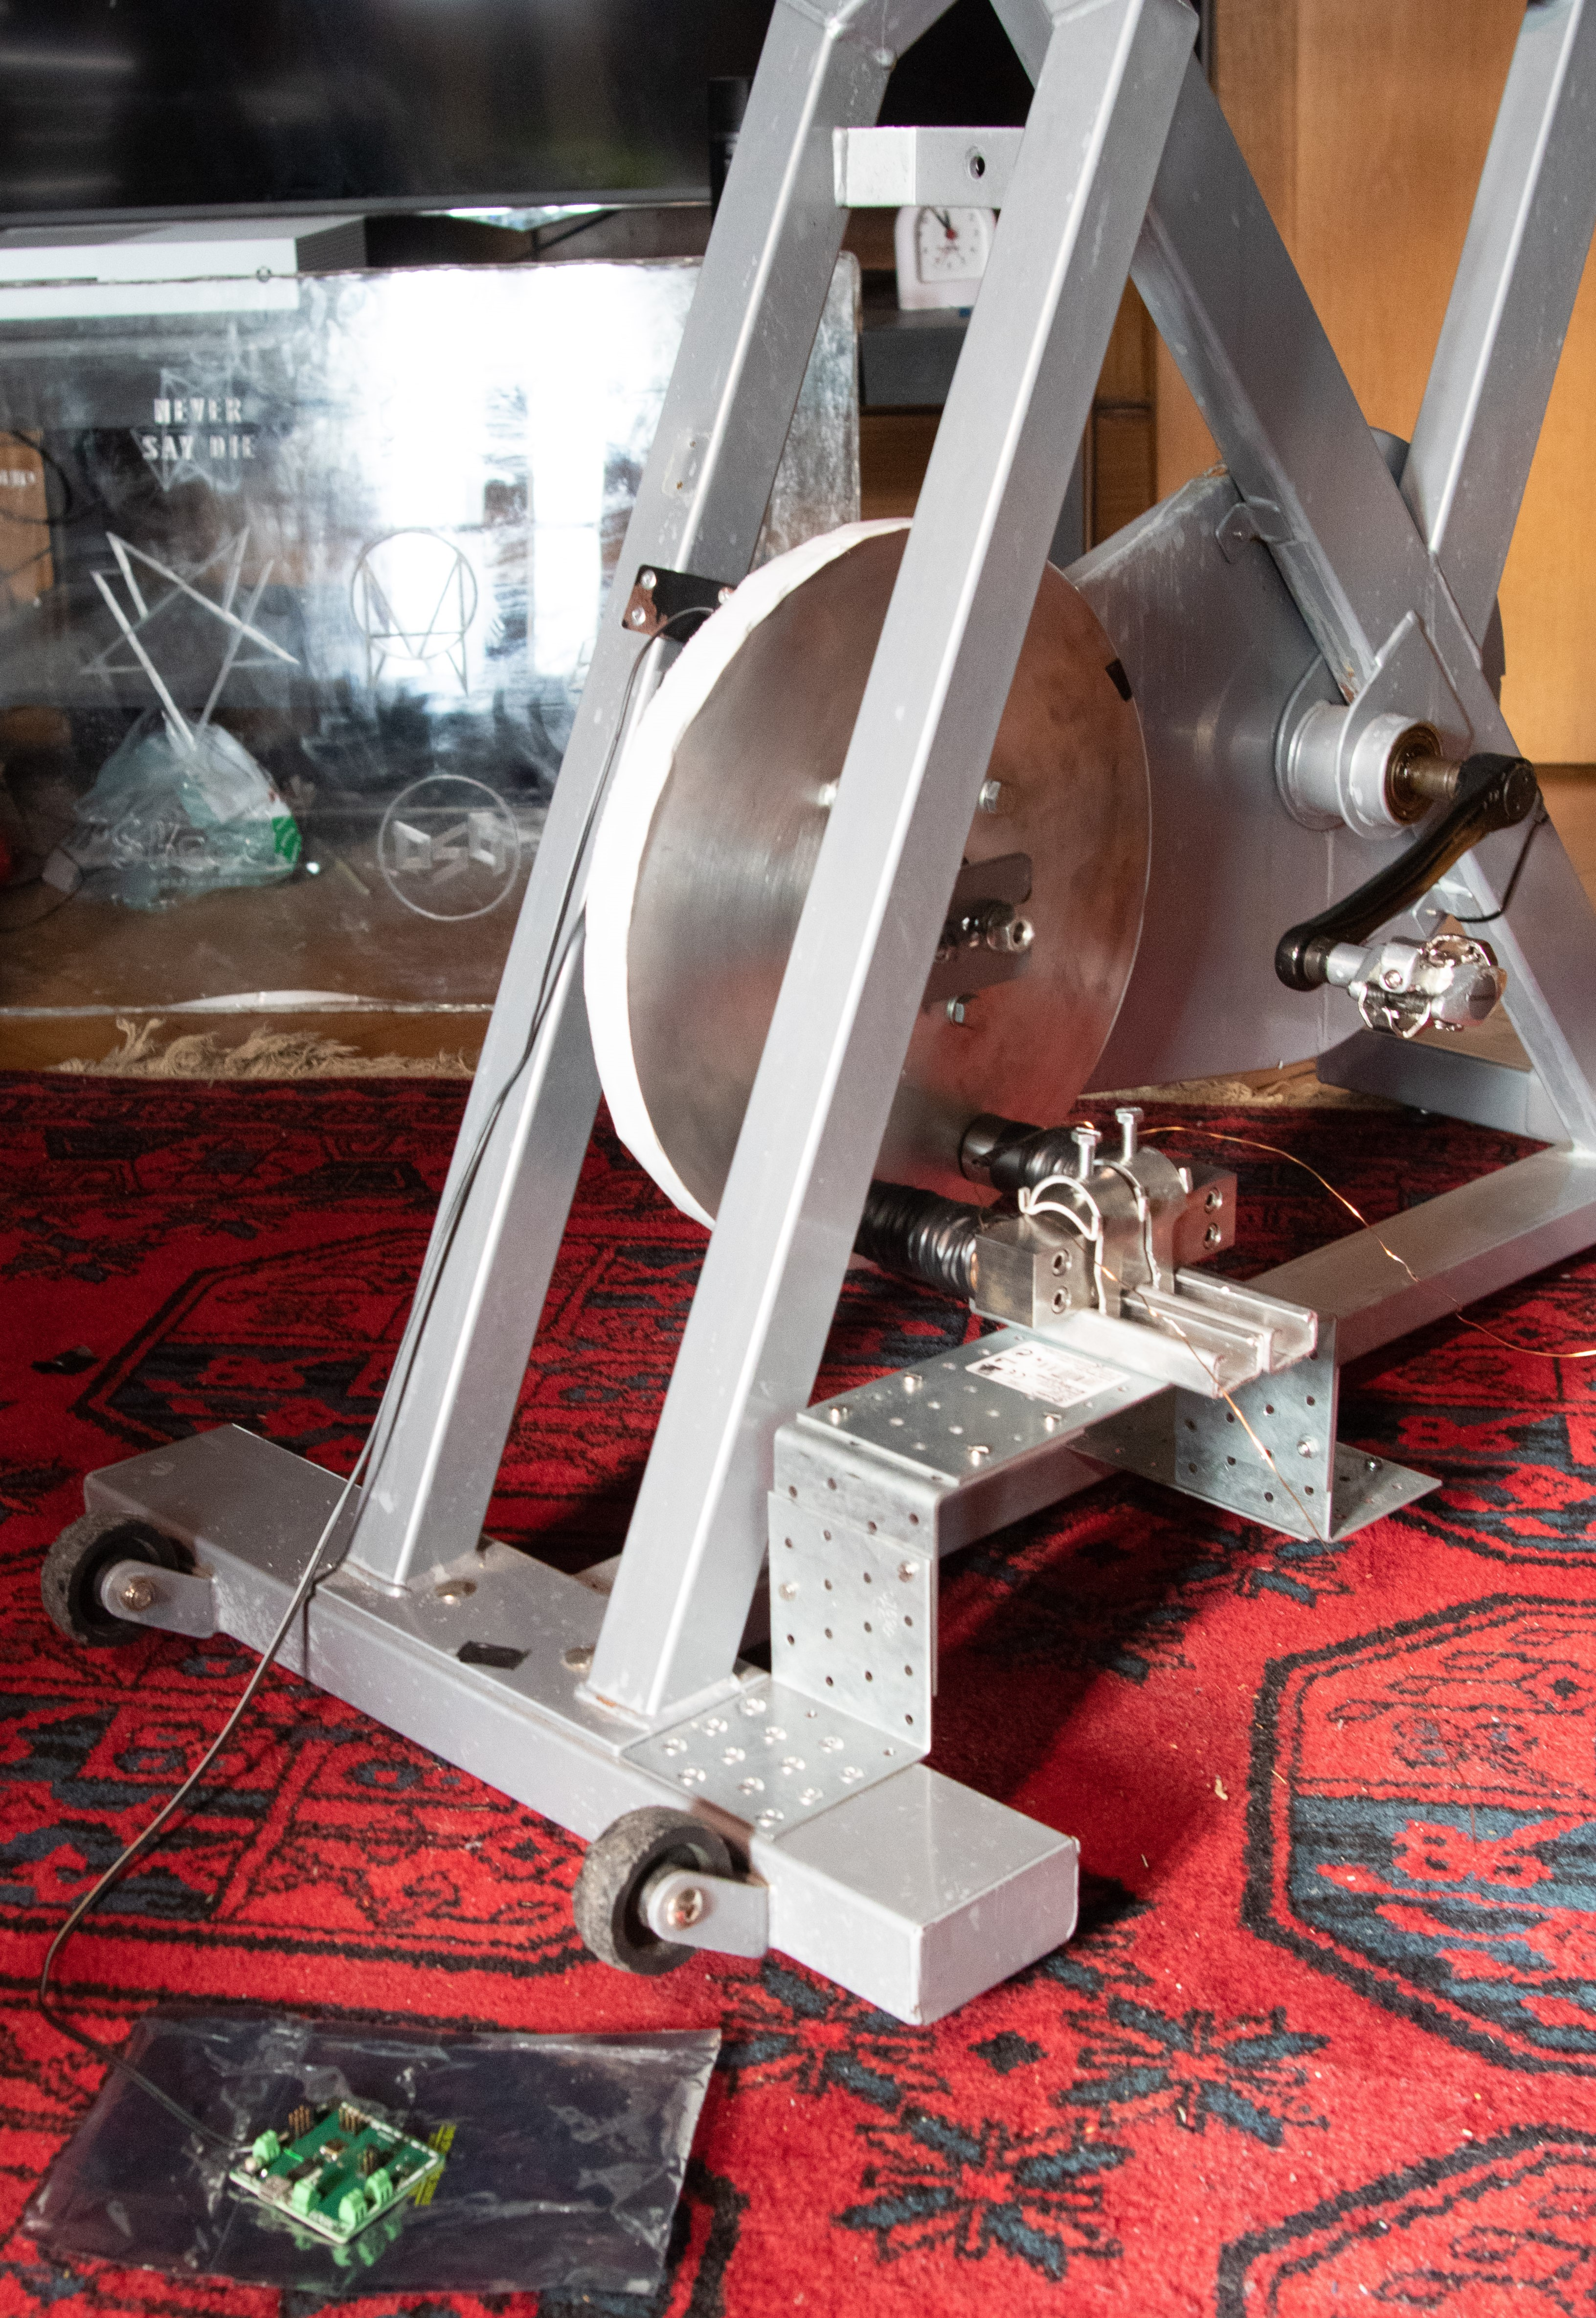
\includegraphics[height=10cm]{assets/images/aufbau/aufbau_magnet}
  \end{center}
  \vspace{-3ex}
  \caption{Gesamtaufbau}
  \label{fig:gesamtaufbau}
\end{figure}
\subsection{Drehzahlmessung} \label{cap:methoden_drehzahlmessung}
Mit der Drehzahlmessung wurde die Genauigkeit der Elektronik gemessen. Diese Genauigkeit wurde mit dem Drehzahlmessgerät überprüft. Da das Messgerät in der Industrie verwendet wird, ist die Messtoleranz sehr klein, führt also zu einem genauen Resultat.
\newpara
Die Drehzahl ist der Kehrwert von der Zeit, welche für eine Umdrehung benötigt wird (Siehe Formel \ref{equ:drehzahl}). Sie gibt an, wie viele Umdrehungen in einer Sekunde gemacht werden können.

\begin{equation}
    \label{equ:drehzahl}
    n=\frac{1}{t} \tag{20}
  \end{equation}
  \begin{gather}
  \shortintertext{\textbf{Begriffe:}}
  \begin{tabularx}{0.9\textwidth}{ll}
    $n$  & Drehzahl\\
    $t$  & Zeit für eine Umdrehung\\
  \end{tabularx}\nonumber
\end{gather}
(\cite[S.86]{kuchling2014taschenbuch})
\newpara
Die Zeit wird mit einem digitalen Timer gemessen, was aber zu einer Einschränkung führt. Diese Einschränkung ist die Speichergrösse des Timers, da dieser begrenzt ist. Das heisst, dass der Timer nur für eine bestimmte Zeit laufen kann, bis dieser sich wieder zurücksetzt. Wenn aber der Timer als eine Art Metronom rekonfiguriert wird, kann ein Intervall mit einem konstanten Rhythmus produziert werden (Siehe Abbildung \ref{fig:plot_timer_verlauf}). 
\newpara
\begin{figure}[h]
  \begin{center}
    \begin{tikzpicture}
      \begin{axis}[
        axis_regulator_style,
               %title         = P-Regler mit konstanter Abweichung,
               ylabel         = {Zählerstand},
               xticklabels    = {,,},
        ylabel near ticks, 
        yticklabel pos        = left,
        minor      grid style = {dashed,gray},
                   ymax       = 23,
                   ymin       = 0,
                   xmax       = 20,
                   xlabel     = {t},
        legend     style      = {draw=none}
      ]
      
        \addplot[line_red] table[x=time,y=value,col sep=comma,mark=none]{assets/diagramm/timer_verlauf.csv}; 
        \addlegendentry{Timer}
      \end{axis}
      \draw[<->](2.90,2.8) -- node[above =0.3cm,font = {\fontsize{8 pt}{16 pt}\selectfont}]{Zeit für ein Inkrement} (3.25,2.8);
      \draw[-](3.25,2.5) -- (3.25,3);
      \draw[-](2.90,2.2) -- (2.90,3);
      \draw[-](5.77,4) -- (5.77,5);
      \draw[<->](0,4.8) -- node[above,font = {\fontsize{8 pt}{16 pt}\selectfont}]{Zeit für ein Interval} (5.77,4.8);
    \end{tikzpicture}
  \end{center}
  \vspace{-3ex}
  
  \caption{Intervall Durchgang des Timers}
  \label{fig:plot_timer_verlauf}
\end{figure}

Nun werden die Intervalle bei einer Umdrehung des Rades gezählt. Man weiss nun anhand der Anzahl Intervallen und des Zählerstandes des Timers, wie lange eine Umdrehung dauert (Siehe Abbildung \ref{equ:zeit_drehzahl}).

\begin{equation}
    \label{equ:zeit_drehzahl}
    t=x_{Z\ddot{a}hler}\cdot t_{Timer}+x_{Intervalle}\cdot t_{Intervalle} \tag{21}
  \end{equation}
  \begin{gather}
  \shortintertext{\textbf{Begriffe:}}
  \begin{tabularx}{0.9\textwidth}{ll}
    $x_{Z\ddot{a}hler}$	     & Zählerstand des Timers (dient für ein genaueres Resultat) \\
    $x_{Intervalle}$	 & Anzahl Intervalle pro Umdrehung \\
    $t_{Timer}$	     & Dauer zwischen zwei Inkrements \textrightarrow 16us \\
    $t_{Intervalle}$	 & Dauer eines Intervalls \textrightarrow $\approx$ 25ms     \\
  \end{tabularx}\nonumber
\end{gather}

Das folgende Diagramm (Siehe Abbildung \ref{fig:plot_timer_magnetschalter_impuls}) zeigt das Verhalten des Timers. Die untere Linie ist der Timer und die obere Linie der Magnetschalter des Rades. Im Verlaufe der Zeit werden mehrere Intervalle gezählt, bis der Magnetschalter einen Impuls erzeugt. Der Timer wird in seinem aktuellen Zustand wieder zurückgesetzt und fängt erneut an zu zählen, bis wieder ein Impuls passiert. Gleichzeitig wird der Zählstand kopiert und abgespeichert, damit dieser vom Mikrocontroller verarbeitet werden konnte.
\newpara
\begin{figure}[h]
  \begin{center}
    \begin{tikzpicture}
      \begin{axis}[
        axis_regulator_style,
               %title         = P-Regler mit konstanter Abweichung,
               yticklabels    = {,,},
               xticklabels    = {,,},
        ylabel near ticks, 
        yticklabel pos        = left,
        minor      grid style = {dashed,gray},
                   ymax       = 10,
                   ymin       = 0,
                   xmax       = 20,
                   xlabel     = {t},
        legend     style      = {draw=none}
      ]
        \addplot[line_blue] table[x=time2,y=value2,col sep=comma,mark=none]{assets/diagramm/timer_durchlauf.csv};       
        \addlegendentry{Magnetschalter}
      
        \addplot[line_red] table[x=time,y=value,col sep=comma,mark=none]{assets/diagramm/timer_durchlauf.csv};    
        \addlegendentry{Timer}
      \end{axis}
      \draw[<->](0,2.7) -- node[above]{Zeit für eine Umdrehung} (5.78,2.7);
      \draw[-,black!70,thick](5.78,0.6) -- (5.78,3.6);
    \end{tikzpicture}
  \end{center}
  \vspace{-3ex}
  
  \caption{Eine Radumdrehung}
  \label{fig:plot_timer_magnetschalter_impuls}
\end{figure}
\newpage

\subsubsection{Messungsaufbau}
Damit bewiesen werden kann, dass die Messung übereinstimmt, muss die Zeit anhand einem Messungsaufbau gemessen und verglichen werden. Dazu wurde das bereits erwähnte Drehzahlmessungsgerät, eine Kamera und ein Laptop verwendet. Mit der Kamera wurde das Display des Drehzahlmessungsgerät aufgenommen, da das Messgerät kein Logger besitzt. Mit dem Laptop wurden die Resultate der Elektronik, welche über USB gesendet wurden, aufgezeichnet.
\newpara
Im Kapitel \ref{cap:methoden_datenauswertung} wird erklärt, wie die Aufnahmen verarbeitet und ausgewertet werden. Wichtig bei dieser Messung ist das Verhältnis des Messgerätes und der Elektronik. Anhand des Verhältnisses ist es möglich, herauszufinden, wie genau die Elektronik im Vergleich zum Messgerät ist. Das Verhältnis wird mit folgender Formel berechnet (Siehe Formel \ref{equ:verhaltnis}).

\begin{equation}
    \label{equ:verhaltnis}
    Verh\ddot{a}ltnis=\frac{n_{Elek}}{n_{Mess}} \tag{22}
  \end{equation}
  \begin{gather}
  \shortintertext{\textbf{Begriffe:}}
  \begin{tabularx}{0.9\textwidth}{ll}
    $n_{Elek}$	     & Drehzahl der Elektronik\\
    $n_{Mess}$	 & Drehzahl des Messgerätes \\
  \end{tabularx}\nonumber
\end{gather}
\subsection{Magnetbremsung} \label{cap:methoden_magnetbremsung}

Der Aufbau ist derselbe wie bei Kapitel \ref{cap:methoden_drehzahlmessung}. Anstatt die Genauigkeit der Drehzahl zu messen, wird die Abbremsung des Rades gemessen. Dabei wird das Rad unterschiedlich beeinflusst, mit eingeschaltetem Magnet und mit ausgeschaltetem Magnet (Leerlauf, ohne Beeinflussung). Werden zwei Messungen gemacht mit ein- und ausgeschaltetem Magnet, kann die Kurve verglichen werden und dadurch kann erkannt werden, ob der Magnet einen Einfluss hat.
\newpara
Die Erwartungen dieser Messung ist das Verhalten der Bremse anhand des Vergleichs (im oberen Paragraphen erwähnt) messen zu können. Im Kapitel \ref{cap:methoden_magnet_design} wird mit der Formel \ref{equ:winkelbeschleunigung} die Winkelbeschleunigung berechnet, welche in dieser Messung zur Auswertung verwendet wird. Wiederum im Kapitel \ref{cap:methoden_magnet_design} wurde erwähnt, dass die gewünschte Winkelbeschleunigung/-abbremsung 1 rad·s-2 entspricht. Die Messresultate der Elektronik müssen daher zuerst in die Winkelbeschleunigung umgewandelt werden. Die Winkelbeschleunigung entspricht der Kreisfrequenzänderung während einer bestimmten Zeit (Siehe Formel \ref{equ:winkelbeschleunigung_magnetbraking}).

\begin{equation}
    \label{equ:winkelbeschleunigung_magnetbraking}
    \alpha=\frac{\Delta\omega}{\Delta t}=\frac{\omega_2-\omega_1}{\Delta t} \tag{23}
  \end{equation}
  \begin{gather}
  \shortintertext{\textbf{Begriffe:}}
  \begin{tabularx}{0.9\textwidth}{ll}
$\alpha$ &	Winkelbeschleunigung\\
$\Delta\omega$    &   Kreisfrequenzänderung während der Zeit $\Delta t$\\
$\Delta t$    &   Zeit während zwei Zeitpunkten (diese Zeit wird in Kapitel (Datenauswertung) berechnet)\\
$\omega_1$    &   Anfangskreisfrequenz\\
$\omega_2$    &   Endkreisfrequenz\\
  \end{tabularx}\nonumber
\end{gather}
(\cite[S.88]{kuchling2014taschenbuch})
\newpara
Wird diese Formel mit der Formel der Winkelfrequenz ($\omega=2\cdot \pi\cdot n$) erweitert, kann die Winkelbeschleunigung mit der Drehzahl berechnet werden (Siehe Formel \ref{equ:winkelbeschleunigung_magnetbraking_erweitert}).
\begin{equation}
    \label{equ:winkelbeschleunigung_magnetbraking_erweitert}
    \alpha=\frac{(2\cdot \pi\cdot n_2)-(\omega=2\cdot \pi\cdot n_1)}{\Delta t}=\frac{2\cdot \pi\cdot(n_2-n_1)}{\Delta t} \tag{24}
  \end{equation}
  \begin{gather}
  \shortintertext{\textbf{Begriffe:}}
  \begin{tabularx}{0.9\textwidth}{ll}
$n_1$    &   Anfangsdrehzahl\\
$n_2$    &   Enddrehzahl\\
  \end{tabularx}\nonumber
\end{gather}


\newpage
\subsection{Radanpassung}\label{cap:methoden_radanpassung}
\begin{figure}[ht]
  \begin{center}
    \includegraphics[width=8cm]{assets/images/rad}
  \end{center}
  \vspace{-3ex}
  \caption{Radanpassung durch Bohrungen}
  \label{fig:radanpassung_bild}
\end{figure}
Nach ersten Bremsversuchen wurde klar, welche hohe kinetische Energie in einem schweren Rad stecken kann. Das massive Rad verzögerte nicht erwartungsgemäss, aufgrund der nicht beachteten Trägheit.
\newpara
Da der maximale Wert des Stromflusses innerhalb der Spulen bereits erreicht wurde, musste eine andere Lösung her. Um eine stärkere Verzögerung zu erzielen, wurde das Gewicht, des zu Beginn vorhandene Schwungrad reduziert. 
\newpara
Der Radius des grösseren Schwungrades wurde auf den Durchmesser der anderen zwei Scheiben angepasst. Dieser Vorgang erfolgte durch Bohrungen entlang dem Umkreis der Bremsscheibe (Siehe Abbildung \ref{fig:radanpassung_bild}). Somit verlor das gesamte Rad ungefähr 60\% an Masse.
\newpara
Durch diesen Gewichtsverlust wird eine deutlich stärkere Verzögerung erwartet.
\newpage
\subsection{Datenauswertung} \label{cap:methoden_datenauswertung}

Anhand eines lauten Geräusches (z.B. Schlag auf den Tisch) können die Aufnahmen von den Kapiteln \ref{cap:methoden_drehzahlmessung} \&  \ref{cap:methoden_magnetbremsung}) in einem Filmbearbeitungsprogramm synchronisiert werden und die Daten herausgelesen werden. Dies ist natürlich kein professioneller Weg, diese Zeit zu überprüfen, aber sie funktionierte einwandfrei, mit den Geräten, welche zur Verfügung standen.
\newpara
Der Vorteil daran ist, dass anhand der Bildrate des Films die Zeiten zwischen zwei Bildern konstant und berechenbar sind. Jede Messungsaufnahme besitzt eine Bildrate von 30 Bildern pro Sekunde. Wird nun eine Sekunde durch 30 geteilt, erhält man die Zeit $0.0\overline{3}s$ (Siehe Formel \ref{equ:time_datenauswertung}).

\begin{equation}
    \label{equ:time_datenauswertung}
    t=\frac{t}{Anzahl Bildern}=\frac{1s}{30}=0.0\overline{3}s \tag{25}
  \end{equation}
  \begin{gather}
  \shortintertext{\textbf{Begriffe:}}
  \begin{tabularx}{0.9\textwidth}{ll}
$n_1$    &   Anfangsdrehzahl\\
$n_2$    &   Enddrehzahl\\
  \end{tabularx}\nonumber
\end{gather}

Als Filmbearbeitungsprogramm wurde Davinci Resolve von Blackmagic-Design verwendet. Wichtig war es, ein Programm zu verwenden, welches ein Projekt als einzelne Bilder exportieren kann. Ein Projekt wird erstellt und die Kamera- und Laptopaufnahme wird in die Medien-Bibliothek aufgenommen. Diese werden nun in die Timeline hineingezogen und aufeinandergelegt. Eine Aufnahme wird solange verschoben, bis alle Geräusche synchron klingen (kein Echo).



\begin{figure}[ht]
    \begin{center}
      \includegraphics[width=14cm]{assets/images/resolve_mediapool}
    \end{center}
    \vspace{-3ex}
    \caption{Ausschnitt aus Davinci Resolve}
    \label{fig:resolve_mediapool}
  \end{figure}

Als Filmbearbeitungsprogramm wurde \textit{Davinci Resolve} von \textit{Blackmagic-Design} verwendet. Wichtig war es, ein Programm zu verwenden, welches ein Projekt als einzelne Bilder exportieren kann. Ein Projekt wird erstellt und die Kamera- und Laptopaufnahme wird in die Medien-Bibliothek aufgenommen. Diese werden nun in die \textit{Timeline} hineingezogen und aufeinandergelegt. Eine Aufnahme wird solange verschoben, bis alle Geräusche synchron klingen (kein Echo) (siehe Abbildung \ref{fig:resolve_mediapool}).
\newpara
Wurde dieser Schritt gemacht, wird das Video als TIFF bei der kleinsten Auflösung (720 x 480 Pixel) exportiert. Als Endprodukt erhält man einzelne Bilder, die je nach Länge des Videos variieren (siehe Formel \ref{equ:anzahl_bilder_resolve}).

\begin{equation}
    \label{equ:anzahl_bilder_resolve}
    Anzahl Bilder=t_{Video}\cdot f_{fps} \tag{26}
  \end{equation}
  \begin{gather}
  \shortintertext{\textbf{Begriffe:}}
  \begin{tabularx}{0.9\textwidth}{ll}
$t_{Video}$    &   Länge des Videos\\
$f_{fps}$    &   Bildrate des Videos\\
  \end{tabularx}\nonumber
\end{gather}
Das längste Video beträgt eine Länge von ca. 3 Minuten, was ca. 5400 Bildern entspricht. Zur Auswertung sind dies zu viele Bildern, da die Werte von Hand in eine Excel Tabelle eingetragen werden müssen. Für dieses Projekt wird es keine gravoeremdem Folgen haben, wenn die Anzahl Bilder gekürzt wird. Es wird daher eine maximale Menge von 250 Bildern pro Messung gesetzt. Bei 250 Bildern können grosse Änderungen immer noch erkannt werden, dafür aber keine Feinänderungen.
\newpara
Werden die exportierten Bilder auf 250 Stück gekürzt, wird sich auch die Zeit zwischen zwei Bildern ändern (Siehe Formel \ref{equ:faktor_bilder} \& \ref{equ:zeit_verlangsamung}). Wird als Beispiel ein Faktor von 32 berechnet und das Video besitzt eine Bildrate von 30 Bildern pro Sekunde, würde eine Zeit von 1.0¯6s berechnet.

\begin{equation}
    \label{equ:faktor_bilder}
    x=\frac{x_{BilderTotal}}{x_{BilderSoll}} \tag{27} 
  \end{equation}
  \begin{equation}
    \label{equ:zeit_verlangsamung}
    t_{fps}=\frac{x}{f_{fps}} \tag{28} 
  \end{equation}
  \begin{gather}
  \shortintertext{\textbf{Begriffe:}}
  \begin{tabularx}{0.9\textwidth}{ll}
    $x$	        &   Bilder-Verkleinerungs-Faktor\\
    $x_{Total}$ &	Totale Anzahl Bilder des exportierten Videos\\
    $x_{Soll}$  &	Gewünschte Anzahl Bilder\\
    $t_{fps}$   &	Zeit zwischen zwei Bildern\\
    $f_{fps}$   &	Bildrate\\
  \end{tabularx}\nonumber
\end{gather}

Sind alle Bilderserien vorbereitet, können die Daten auf den Bildern in ein Excel eingetragen werden und verarbeitet werden.
\newpage
\subsection{Magnetansteuerung - Konzept} \label{cap:methoden_magnetansteuerung}
Dieses Kapitel gilt als Konzept, da anhand Fehlberechnungen, Zeitdruck und Vergleichung gemessener Werte die Umsetzung dieser Methode nicht möglich war.
\newpara

Das Magnet würde mit einem PWM-Signal angesteuert werden, was uns erlaubt, das Magnet unterschiedlich stark anzusteuern. PWM, Pulse-Width-Modulation, ist in der Elektronikwelt weit verbreitet, z.B. in LED-Lampen mit verstellbarer Helligkeit. Bei einem PWM-Signal wird ein Element eine bestimmte Zeit lang ein- und ausgeschaltet, wobei das Verhältnis zwischen diesen beiden Zeiten als Tastgrad angegeben wird. Der Tastgrad gibt in Prozent an, wie lange das Element während einer Periode eingeschaltet bleibt. In anderen Worten, der Tastgrad gibt an, wie viel von der maximalen Energie der Magnet erhält (Siehe Abbildung \ref{fig:plot_pwm}).
\newpara
\begin{figure}[h]
  \begin{center}
    \begin{tikzpicture}
      \begin{axis}[
        axis_regulator_style,
               %title         = P-Regler mit konstanter Abweichung,
               ylabel         = {Spannung},
               y unit         = {V},
        ylabel near ticks, 
        yticklabel pos        = left,
        minor      grid style = {dashed,gray},
                   ymax       = 2,
                   ymin       = 0,
                   xmax       = 20,
                   xlabel     = {t},
                   xticklabels    = {,,},
        legend     style      = {draw=none}
      ]
      
        \addplot[line_red] table[x=time,y=value,col sep=comma,mark=none]{assets/diagramm/pwm.csv};
        \addlegendentry{PWM-Verlauf}
      \end{axis}
      \draw[<->](0.37,2) -- node[above]{Pause} (2.88,2);
      \draw[<->](2.90,2) -- node[right =0.3cm]{Impuls} (3.60,2);
      \draw[-](0.37,3) -- (0.37,4);
      \draw[-](3.62,3) -- (3.62,4);
      \draw[<->](0.37,3.8) -- node[above]{Periode} (3.62,3.8);
    \end{tikzpicture}
  \end{center}
  \vspace{-3ex}
  
  \caption{PWM Darstellung}
  \label{fig:plot_pwm}
\end{figure}
\newpara
In Kombination mit dem Regler wäre es dann möglich, je nach Abweichung und Regler-Werten, den Magneten unterschiedlich stark anzusteuern.
\newpage
\section{Ergebnisse}\label{cap:ergebnisse}
\subsection{Drehzahlmessung} \label{cap:ergebnisse_drehzahlmessung}
\begin{figure}[ht]
    \begin{center}
      \begin{tikzpicture}
        \begin{axis}[
          width             = 10cm,
          compat            = 1.3,
          axis y line*      = left,
          ylabel            = {Drehzahl},
          xlabel            = {Zeit},
          legend pos        = south east,
          legend cell align = {left},
          x unit            = {\si{\second}},
          y unit            = {\si{1\per\second}},
          legend style      = {draw=none}
        ]
        
          \addplot[line_red] table[x= time,y=electronic,col sep=comma,mark=none]{assets/messurement_results/tempo.csv}; 
          \label{plot:tempo_electronic}           
          \addlegendentry{Drehzahl Elektronik}
        
          \addplot[line_blue] table[x= time,y=mess_converted,col sep=comma,mark=none]{assets/messurement_results/tempo.csv}; 
          \label{plot:tempo_measured}
          \addlegendentry{Drehzahl Messgerät}
        \end{axis}
        \begin{axis}[
          compat            = 1.3,
          width             = 10cm,
          axis y line*      = right,
          axis x line       = none,
          ylabel            = {Verhältnis},
          ymin              = 0,
          ymax              = 2,
          legend pos        = south east,
          legend cell align = {left},
          legend style      = {draw = none}
        ]
          \addlegendimage{/pgfplots/refstyle=plot:tempo_electronic}\addlegendentry{Drehzahl Elektronik}
          \addlegendimage{/pgfplots/refstyle=plot:tempo_measured}\addlegendentry{Drehzahl Messgerät}

          \addplot[line_black] table[x= time,y=ratio_el_me,col sep=comma,mark=none]{assets/messurement_results/tempo.csv}; 
          \label{plot:tempo_ratio}     
          \addlegendentry{Verhältnis}
        \end{axis}
      \end{tikzpicture}
    \end{center}
    \vspace{-3ex}
    
    \caption{Resultat der Messung}
            
    \label{fig:tempo_measurement}
  \end{figure}

  Als Vorgabe wurde eine Toleranz von $\pm$ 5\% der Drehzahl geplant. Diese Vorgabe scheint die Elektronik einzuhalten. Im rechten Bereich (ab Sekunde 15) ist das Verhältnis der beiden Messresultaten sehr nahe, wobei im linken Bereich (ab Sekunde 0 bis 15) die Eigenschaft des Messgerätes das Verhältnis stark verfälscht. Das Messgerät misst die Anzahl Pulse während einer Sekunde und berechnet daraus die Drehzahl. Die Elektronik misst die Zeit zwischen zwei Pulsen und berechnet daraus die Drehzahl.

\newpage
\subsection{Magnetbremsung}\label{cap:ergebnisse_magnetbremsung}
\subsubsection{Vor Radanpassung}
\begin{figure}[ht]
  \begin{center}
    \begin{tikzpicture}
      \begin{axis}[
        axis_results_style,
        ylabel            = {Drehzahl},
        xlabel            = {Zeit},
        ymax              = 12,
        ymin              = 0,
        xmax              = 220,
        xmin              = 0,
        legend style      = {draw=none},
        ylabel near ticks, 
        extra x ticks=0,
        x unit            = {\si{\second}},
        y unit            = {\si{1\per\second}},
      ]
        \addplot[line_blue] table[x= time,y=electronic,col sep=comma,mark=none]{assets/messurement_results/ohne_mag_ohne_rad.csv}; 
        \label{plot:omor_electronic}
        \addlegendentry{Ohne Magnet}
        \addplot[line_red] table[x= time,y=electronic,col sep=comma,mark=none]{assets/messurement_results/mit_mag_ohne_rad.csv}; 
        \label{plot:imor_electronic}
        \addlegendentry{Mit Magnet}
      \end{axis}
    \end{tikzpicture}
  \end{center}
  \vspace{-3ex}
  \caption{Resultat Ohne \& Mit Magnet, Vor Anpassung bei 4A}
  \label{fig:plot_or_results}
\end{figure}
Die Messung wurde mit 4A anstatt 2A gemacht, da bei 4A die Änderungen besser erkannt werden kann.
\newpara
Als Vorgabe war die im Kapitel \ref{cap:methoden_magnet_design} erwähnten Winkelbeschleunigung einzuhalten (1 $rad\cdot s^{-2}$). Diese scheint anhand dieser Messung (Siehe Abbildung \ref{fig:plot_or_results}) diese Vorgabe nicht einzuhalten. Der Grund dafür sind die Trägheit des Rades und daher auch eine Fehlberechnung des Magneten. Nach Überprüfung der Berechnungen wurde herausgefunden, dass nicht nur das Gewicht der Bremsscheibe einzuberechnen war, sondern auch allen Elementen, die an dieser Scheibe befestigt waren. Anhand dieser Erkenntnis wurde die im Kapitel \ref{cap:methoden_radanpassung} erwähnten Anpassung ausgeführt.
\newpara
Zu erkennen ist der Effekt des Wirbelstroms im Magnetbetrieb. Ab Sekunde 60 fängt das System schwächer zu Bremsen.

\newpage
\subsubsection{Nach Radanpassung}
\begin{figure}[ht]
  \begin{center}
    \begin{tikzpicture}
      \begin{axis}[
        axis_results_style,
        ylabel            = {Drehzahl},
        xlabel            = {Zeit},
        ymax              = 20,
        ymin              = 0,
        xmax              = 70,
        xmin              = 0,
        legend style      = {draw=none},
        ylabel near ticks, 
        extra x ticks=0,
        x unit            = {\si{\second}},
        y unit            = {\si{1\per\second}},
      ]
        \addplot[line_blue] table[x=time,y=electronic,col sep=comma,mark=none]{assets/messurement_results/ommr.csv};
        \label{plot:omir_electronic}
        \addlegendentry{Ohne Magnet}
        \addplot[line_red] table[x= time,y=electronic,col sep=comma,mark=none]{assets/messurement_results/mit_mag_mit_rad.csv}; 
        \label{plot:imir_electronic}
        \addlegendentry{Mit Magnet}
      \end{axis}
    \end{tikzpicture}
  \end{center}
  \vspace{-3ex}
  \caption{Resultat Ohne \& Mit Magnet, Nach Anpassung bei 4A}
  \label{fig:plot_ir_results}
\end{figure}
Die Messung wurde mit 4A anstatt 2A gemacht, da bei 4A die Änderungen besser erkannt werden kann.
\newpara
Die allgemeine Abbremsung konnte um ein dreifaches gekürzt werden (ca. 12kg Metall konnte entfernt werden). Die Winkelbeschleunigung dieser Messung ist sehr nahe der erwartenden Abbremsung. Der Knick in der Magnetbremsung ab Sekunde 7 repräsentiert den Zeitpunkt, wo der Magnet eingeschaltet wurde. Wiederum kann die schwächere Bremsung gegen Ende der Magnetbremsung erkannt werden.
\newpage
\section{Diskussionen} \label{cap:diskussion}
\subsection{Drehzahlmessung}\label{cap:diskussion_drehzahlmessung}
Die Ergebnisse der Messung sind zufriedenstellend. Es war möglich, die Drehzahl genau messen zu können. Die Grundstruktur des Drehzahlmessers ist in einem guten Zustand und kann als Grundbaustein für ein zukünftiges Model der Wirbelstrombremse dienen. Die Messung übertrafen die Erwartungen und konnte in den anderen Messungen erfolgreich eingesetzt werden.
\newpara
Der einzige Nachteil, welcher nicht in den Resultaten erkannt wurde, waren schwankende Messwerte. Während der Programmierung hatte der Drehzahlmesser Probleme mit den Reaktionen. Der gemessene Wert schwankte oft im Bereich von ±2.5ms von der realen Drehzahl. Dies konnte während der Entwicklung auf ca. ±0.2ms reduziert werden.
\newpara
Als Version 1 der Bremse reicht die Messung, aber für Version 2 oder 3 wird sich die Genauigkeit verbessern müssen und die Schwankungen müssten auch möglichst gelöst werden. 
\subsection{Magnetbremsung}\label{cap:diskussion_magnetbremsung}
Zu Beginn waren die Resultate nicht zufriedenstellend. Es drehte zu langsam, nicht nach den Projektvorgaben. Die Resultate galten daher als unbrauchbar. Nachdem erkannt wurde, dass die langsame Geschwindigkeit des Rades durch die Trägheit der Bremsscheibe und des Fitnessrades, an welchem die Bremsscheibe befestigt wurde, beeinflussten, wurde das Rad angepasst. 
\newpara
Nach der Anpassung waren die Messungen zufriedenstellender, aber nicht dennoch gemäss Erwartungen. Nach den Vorstellungen hätte die Bremse einer in praktischen Bereichen eingesetzten Wirbelstrombremse ähneln müssen. Die Vorgaben waren zu unterdimensioniert und die Wirbelstrombremse reagierte daher zu langsam. Die Resultate galten wiederum als unzufriedenstellend.
\newpara
Ein gutes Zeichen aber war, dass der Magnet funktionierte. Nur durch Entfernen von ca. 12kg Metall konnte eine Verdreifachung der Abbremsung erkannt werden. Daraus konnten einige Erkenntnisse gezogen werden. Der Magnet ist abhängig von der Last, die der Magnet bremsen muss, und durch Verkleinerung dieser Last verbessert sich die Bremskraft. Dies ist ein Meilenstein des Projekts. Man kann anhand dieser Erkenntnisse das Magnet neu dimensionieren und den Aufbau der Wirbelstrombremse neu aufbauen.
\newpage
\subsection{Nichterreichung}
Die Erreichung der Hypothese konnte aus folgenden Gründen nicht erreicht werden:
\begin{itemize}
  \item Fehlberechnungen
  \item Kenntnis über Regler
  \item Zeitdruck
\end{itemize}
\subsubsection{Fehlberechnungen}
Bereits im Kapitel \ref{cap:methoden_magnet_design} erwähnt, wurden die Formeln falsch angewendet. Dies hat den Grund, dass mit dem \textit{Trail-\&-Error}-Prinzip der Magnet dimensioniert wurde. Das Trägheitsdrehmoment und das Drehmoment von W.R. Smythes Formel \ref{equ:smythe_rotation_included} wurden nur miteinander verglichen, anstatt zusammenzuführen. Dies hat den Nachteil, dass der Magnet zu ungenau dimensioniert wird. Folgend wird die korrekte Zusammenstellung der Formel aufgeführt.
\newpara
Wird anhand den aufgelisteten Formeln im Kapitel \ref{cap:methoden_magnet_design} eine einzige Formel erstellt, würde die Berechnung des Magneten stark vereinfacht. Die Formel (\ref{equ:smythe_rotation_included}) wird mit den Formeln \ref{equ:magnetischer_fluss}, \ref{equ:magnetische_durchflutung}, \ref{equ:magnetischer_widerstand}, \ref{equ:magnetischer_serie_widerstand} und \ref{equ:tragheitsmoment_kombiniert} erweitert, damit kann eine einzige  Formel erstellt werden. Die daraus folgende Formel beinhaltet alle benötigten Parameter, welche für die Dimensionierung verwendet wird (Siehe Formel ).

\begin{equation}
  \label{equ:smythe_tragheit_kombiniert}
  \frac{m\cdot r^{2}\cdot \Delta\omega}{\Delta t}=\frac{n_{MAX}\cdot b\cdot \gamma\cdot (\frac{N\cdot I}{R_M})^{2}\cdot c^{2}}{a^{2}} \cdot (1-\frac{A^{2}\cdot a^{2}}{(A^{2}-c^{2})^{2}}) \tag{29}
\end{equation}
\newpara
Wird nach $R_M$ aufgelöst, erhält man (Formel \ref{equ:smythe_tragheit_RM_aufgelost})

\begin{equation}
  \label{equ:smythe_tragheit_RM_aufgelost}
  R_{M}=\frac{c\cdot I \cdot N}{a \cdot r}\cdot \frac{\sqrt{\Delta t \cdot n_{MAX}\cdot b \cdot \gamma \cdot (1-\frac{A^{2}\cdot a^{2}}{(A^{2}-c^{2})^{2}})}}{\sqrt{m\cdot\Delta\omega}} \tag{30}
\end{equation}
\newpara

$R_{M}$ beinhaltet Informationen über die Grösse des Magneten, der Aluminiumscheibe und des Luftspalts. Formel \ref{equ:magnetischer_serie_widerstand} wird mit der Formel des magnetischen Widerstands \ref{equ:magnetischer_widerstand} für den Luftspalt, für  die Aluminiumscheibe und für den Magneten erweitert (Siehe Formel \ref{equ:magnetischer_widerstand_eingesetzt}).

\begin{equation}
  \label{equ:magnetischer_widerstand_eingesetzt}
R_{M}=\frac{l_{Luft}}{\mu_{0}\cdot A}+\frac{l_{Alu}}{\mu_{0}\cdot \mu_{rAlu}\cdot A}+\frac{l_{Magnet}}{\mu_{0}\cdot \mu_{rMagnet}\cdot A} \tag{31}
\end{equation}
\newpara

Wird die Formel nach $l_{Magnet}$ aufgelöst, erhält man:

\begin{equation}
  l_{Magnet}=\frac{(R_{M}\cdot\mu_{0}\cdot\mu_{rAlu}\cdot A - l_{Luft}\cdot\mu_{rAlu}-l_{Alu})\cdot\mu_{rMagnet}}{\mu_{rAlu}} \tag{32}
\end{equation}
\newpara
Diese Formel ermöglicht nun, durch eine gemeinsame Querschnittsfläche, die Dicke der Scheibe und die Dicke des Luftspalts, die Magnetkreislänge zu berechnen. Anhand Magnetkreislänge und der Querschnittsfläche kann der Magnet dimensioniert werden.
\newpage
\subsubsection{Kenntnis über Regler}
Das zweite Problem geschah beim Austesten des Reglers. Beim Austesten wurden die berechneten Werte des Reglers aufgefangen und am Laptop angezeigt. Nur war nicht bekannt, was funktionsweise richtig war. Die im Anhang hinterlegten Tabelle mit dem Name \textit{results\_regler\_messung} zeigt Regelwerte im Bereich von 700 bis 800 an, was als zu hoch gilt. Diese Werte wurden anhand einem kleinen Test ermittelt, worin das Ziel war, den PID-Regler der Elektronik auszuprobieren (Siehe Abbildung \ref{fig:pid_regler_plot}).

\begin{figure}[ht]
    \begin{center}
      \begin{tikzpicture}
        \begin{axis}[
          width             = 12cm,
          compat            = 1.3,
          axis y line*      = left,
          ylabel            = {Drehzahl},
          xlabel            = {Zeit},
          legend pos        = north east,
          legend cell align = {left},
          x unit            = {\si{\second}},
          y unit            = {\si{1\per\second}},
          legend style      = {draw=none},
          xmax              = 40
        ]
        
          \addplot[line_red] table[x= time,y=electronic,col sep=comma,mark=none]{assets/diagramm/diskussion/pid_regler.csv}; 
          \label{plot:ist_drehzahl}           
          \addlegendentry{Ist-Drehzahl}
        
          \addplot[line_blue] table[x= time,y=solldrehzahl,col sep=comma,mark=none]{assets/diagramm/diskussion/pid_regler.csv}; 
          \label{plot:soll_drehzahl}
          \addlegendentry{Soll-Drehzahl}
        \end{axis}
        \begin{axis}[
          compat            = 1.3,
          width             = 12cm,
          axis y line*      = right,
          axis x line       = none,
          ylabel            = {Regelwert},
          ymin              = 680,
          ymax              = 760,
          xmax              = 100,
          legend pos        = north east,
          legend cell align = {left},
          legend style      = {draw = none},
          xmax              = 40
        ]
          \addlegendimage{/pgfplots/refstyle=plot:ist_drehzahl,color=red!70,line width= 1pt}
          \addlegendentry{Ist-Drehzahl}
          \addlegendimage{/pgfplots/refstyle=plot:soll_drehzahl,color=blue!70,line width= 1pt}
          \addlegendentry{Soll-Drehzahl}
          \addplot[line_black] table[x= time,y=pid_value,col sep=comma,mark=none]{assets/diagramm/diskussion/pid_regler.csv};
          \label{plot:regelwert_out}     
          \addlegendentry{Regelwert}
        \end{axis}
      \end{tikzpicture}
    \end{center}
    \vspace{-3ex}
    
    \caption{PID-Regelwerte mit Sollwert}
            
    \label{fig:pid_regler_plot}
  \end{figure}

Es kann in der Abbildung \ref{fig:pid_regler_plot} erkannt werden, dass der Regelwert abnimmt, obwohl die Drehzahl zunimmt (bei einer Zunahme müsste der Regelwert zunehmen). 
\newpara
Vermutlich sind die Grössen der Faktoren falsch gesetzt. Diese Werte konnten wegen zu wenig Zeit nicht geändert werden. Es gibt Rechenmethoden, welche für die Dimensionierung der Faktoren verwendet werden könnten, aber schlussendlich wird es mit dem Trial-\&-Error Prinzip enden. Es wird solange ausprobiert, bis geeignete Werte ermittelt werden können.
\newpara
Eine andere Vermutung ist, dass der Regler falsch implementiert wurde oder der verwendete Mikrocontroller die Werte nicht korrekt berechnet. 
\newpara
Der PID-Regler könnte in Zukunft anhand einer berechenbaren Situation überprüft werden. Dies wäre der Plan gewesen für diese Arbeit, aber da die Zeit nicht mehr reichte, wurde dies für die Zukunft geplant.

\subsubsection{Zeitdruck}
Der Hauptgrund, dass die Hypothese nicht erreicht werden konnte, war der Zeitdruck.
\newpara
Der Zeitplan, welcher für die Arbeit erstellt wurde, hat jeden einzelnen Schritt aufgelistet, welcher für die Arbeit ausgeführt werden muss, ausser die Radanpassung, welche während der der Arbeit dazwischen kam. Lieferzeiten und Fehlerbehebungen wurden ebenfalls nicht einberechnet, obwohl diese Schritte eigentlich wichtig sind.
\newpara
In anderen Worten, es kam zum Zeitdruck wegen einer Fehlplanung. Man hätte jeden Schritt detaillierter beschrieben sollen, worin der Ausführende direkt weiss, was gemacht werden muss. Dazu müsste die Planung für die Arbeit länger dauern und bis ins Detail geplant werden. Da dies bei der Arbeit nicht immer der Fall war, wurde zu viel Zeit verloren gegangen und als Folge kam es zum Stress.
\newpara
In Zukunft sollte genügend Zeit für die Planung investiert werden. Jeder Schritt müsste eine Beschreibung, Ziel und geschätzte Verarbeitungszeit besitzen, dass in der gesamten Zeitplanung die Schritte richtig verteilt werden können.

\subsection{Schlussfolgerung}
Der aktuelle Stand der Wirbelstrombremse kann die Geschwindigkeit des Rades messen und die Bremsung selbst ausführen. Es wurde erkannt, dass die Masse, welche an der Bremsscheibe befestigt ist, die Bremsung stark beeinflusst. Die Dimensionierung des Magneten kann anhand W.R. Smythes Formel (Formel \ref{equ:smythe_orignal}) und dem Trägheitsdrehmoment berechnet werden.
\newpara
Anhand diesen Erkenntnissen können mit folgenden Schritten weiter gearbeitet werden:
\begin{itemize}
  \item \textbf{Neue Hardware} - Die Elektronik muss neu designt werden, da die aktuelle Elektronik das Magnet nicht richtig ansteuern kann, weil der Regler nicht richtig funktioniert. Annahme ist, dass der Mikrocontroller zu langsam oder die Berechnungen nicht richtig ausführen kann. Ebenfalls muss der MOSFET ersetzt werden, da nach Austesten der Scheibe mit einer Stromstärke von 4A die Strombegrenzung des MOSFETs überschreitet.
  \item \textbf{Neuer Aufbau} - Insbesondere muss das Rad des Fitnesstrainers durch eine Aluminiumscheibe ersetzt werden. Das Gewicht des Rades hat die Brems zu stark belastet (das Gewicht wurde nicht einberechnet).
  \item \textbf{Besserer Messungsaufbau} - Der Messungsaufbau muss durch bessere Messgeräte ersetzt werden, welche ein Logging-System besitzen. Ein Logging-System ist ein System, welches Daten in bestimmten Intervallen abspeichert, welche man danach digital ablesen kann.
\end{itemize}

\section{Schlusswort} \label{cap:schlusswort}

\subsection{Joel von Rotz}
<< Durch diese Arbeit konnten wir neue Erfahrungen sammeln, welche uns im Berufsleben hilfreich sein können. Wir konnten schlussendlich durch eine umfangreiche Planung eine Wirbelstrombremse entwickeln, welche zwar nicht unseren Erwartungen entsprach, aber dafür neue Kenntnisse, insbesondere über Wirbelstrom und Magnetismus, brachte.
\newpara
Ich erlernte durch diese Arbeit das Dokumentationprogramm \textit{LATEX}. Mit diesem Programm können professionelle Arbeiten geschrieben werden und ich konnte diese Arbeit damit schreiben. Zusätzlich konnte ich einen Magneten anhand mathematischen Formeln berechnen und neue Erkenntnisse im Projektmanagement erlernen. 
\newpara
Mit den neuen Erkenntnissen bin ich bereit, dieses Projekt weiterzuführen. Ich werde bestehende Funktionen verbessern und neue Funktionen in das Projekt implementieren. Ich glaube daran, dass diese Arbeit mir auch in Zukunft neue Erfahrungen bringen wird, welche in weitere Projekte eingesetzt werden können.
\newpara
Trotz dieses Erfahrungserfolg, gerieten wir in Zeitdruck. Wir mussten zusammen innert kürzester Zeit eine Dokumentation  schreiben. Meine Lehre daraus ist, dass ich in Zukunft eine umfangreichere Planung erstellen werde. Reflektiv war dieses Projekt meiner Meinung nach eine gute Lehre, aus Fehlern zu lernen und auch neue Methoden aufzustellen, welche diese Fehler beheben können.
\newpara 
Meinen Erwartungen nach wollte ich die Arbeit vollständig abschliessen, was aber nicht möglich war. Ich bin daher über den Fortschritt nicht ganz zufrieden. Wir konnten einen Meilenstein setzen und ich will diesen weiterführen. 
>>
\subsection{Stefan Ruckli}
<< Unsere Arbeit wandelte sich von einer Grundidee zu einem Projekt, in dem jeder von uns gefragt war. Wir konstruierten schlussendlich eine funktionsfähige Wirbelstrombremse. Hiermit können wir von uns selbst behaupten, dass wenn ein elektrisch Leitfähiges Medium bei Bewegung, welches unter Einfluss eines äusseren Magnetfeld steht, darauf eine Kraft gegen die Bewegung bildet.
\newpara
Ich erwartete von unserem Projekt, dass wir durch Messungen effektiv einen Nachweis über diesen Physikalischen Effekt darlegen können. Dies war bei unserem Projekt durchaus der Fall, was mich faszinierte. Somit setzte ich mich auch gerne mit dem Konzept einer Wirbelstrombremse auseinander. Ich habe viele neue Erfahrungen im Bereich der Elektrotechnik. Darüber hinaus habe ich noch neue Kenntnisse in dem Bereich der Werkstück-Bearbeitung gesammelt.
\newpage
Für mich war die Arbeit, trotz unseres nicht komplett erfüllten Leitsatzes, ein Erfolg. Reflektiv kann ich behaupten, dass unser Projekt jede Erfahrung wert war. >>
\subsection{Filip Estermann}
<< Am Anfang unserer IDPA kannten wir uns noch nicht. Das Einzige, was wir voneinander wussten, war das gemeinsame Interesse an der Elektrizität. Aus diesem Interesse entstanden einige Ideen für unsere Arbeit und schliesslich entwickelte sich daraus ein Projekt. Wir waren alle motiviert, eine gute Arbeit zu machen und wir setzten uns hohe Ziele. Diese waren am Anfang etwas zu gross und wir reduzierten sie für unsere IDPA auf zwei Ziele, die zusammen eine überschaubare Arbeit werden sollen.
\newpara
Meine persönlichen Erwartungen an diese Arbeit waren grösser, als nur unsere Ziele zu erreichen. Ich wollte neue Erfahrungen im Bereich der Elektrotechnik sammeln und mich vor allem bei der Dokumentation weiterentwickeln, da ich bis jetzt noch nie eine solche geschrieben hatte. 
\newpara
Rückblickend kann ich sagen, dass unsere Arbeit ein voller Erfolg war. Wir konnten gut zusammenarbeiten und wir fanden auf auftretende Probleme meistens schnell eine Lösung. Auch wenn wir unser zweites Ziel nicht erreichten, konnten wir daraus trotzdem einiges lernen und es ist eine wertvolle Erfahrung. Meine Erwartungen konnte ich vollständig erfüllen. >>
\newpage

\input{assets/kapitel/10_abbildungsverzeichnis.tex}
\newpage

\input{assets/kapitel/11_glossar.tex}
\newpage

\input{assets/kapitel/12_literaturverzeichnis.tex}
\newpage

\section{Anhang}
\subsection{Eidesstattliche Erklärung}
Wir erklären hiermit, dass wir die vorliegende interdisziplinäre Projektarbeit eigenständig und ohne unerlaubte fremde Hilfe erstellt haben und dass alle Quellen, Hilfsmittel und Internetseiten wahrheitsgetreu verwendet wurden und belegt sind.
\vskip 3cm
[Ort, Datum, Unterschrift]

\subsection{QR-Codes}
Im folgenden Link und QR-Code kann auf sämtliche Anhänge zugegriffen werden.
\vskip 1cm
\qrcode[height=4cm]{https://github.com/joelvonrotz/Eddy-Current-Brake-Regulator}
\newpara
\url{https://github.com/joelvonrotz/Eddy-Current-Brake-Regulator}
\end{document}



% https://www.latextemplates.com/template/formal-book-title-page - template



